\chapter{Géométrie plane} \label{Geo5}

\begin{prerequis}[Dans les programmes - cycle 1]
\small{\bf Explorer des formes - Ce qui est attendu des enfants en fin d'école maternelle}
   \begin{itemize}
      \item Classer des objets en focntion de caractéristiques liées à leur forme.
      \item Savoir nommer quelques formes planes (carré, triangle, cercle ou disque, rectangle) et ce dans toutes les orientations et configurations.
      \item Reproduire un assemblage à partir d'un modèle (puzzle, pavage, assemblage de solides).
      \item Reproduire, dessiner des formes planes.
   \end{itemize}
\end{prerequis}

\begin{prerequis}[Dans les programmes - cycle 2]
\small      {\bf Reconnaitre, nommer, décrire, reproduire quelques figures géométriques. Reconnaitre et utiliser les notions d’alignement, d’angle droit, d’égalité de longueurs, de milieu, de symétrie}
   \begin{itemize}
      \item Décrire, reproduire sur papier quadrillé ou uni des figures ou des assemblages de figures planes.
      \item Utiliser la règle, le compas ou l’équerre comme instruments de tracé.
      \item Reconnaitre, nommer les figures usuelles : carré, rectangle, triangle, triangle rectangle, polygone, cercle, disque.
      \item Décrire à partir des côtés et des angles droits, un carré, un rectangle, un triangle rectangle. Les construire sur un support uni connaissant la longueur des côtés.
      \item Construire un cercle connaissant son centre et un point, ou son centre et son rayon.
      
      \item Utiliser la règle (non graduée) pour repérer et produire des alignements.
      \item Repérer et produire des angles droits à l’aide d’un gabarit, d’une équerre.
      \item Reporter une longueur sur une droite déjà tracée.
      \item Repérer ou trouver le milieu d’un segment.
      \item Reconnaitre si une figure présente un axe de symétrie.
      \item Reconnaître dans son environnement des situations modélisables par la symétrie.
      \item Compléter une figure pour qu’elle soit symétrique par rapport à un axe donné.
   \end{itemize}
\end{prerequis}

\begin{prerequis}[Dans les programmes - cycle 3]
\small   {\bf Reconnaitre, nommer, décrire, reproduire, représenter, construire quelques figures géométriques}
   \begin{itemize}
      \item Reconnaître, nommer, décrire des figures simples ou complexes : triangles, quadrilatères, cercle, disque.
      \item Reproduire, représenter, construire des figures simples ou complexes.
      \item Réaliser, compléter, rédiger un programme de construction.
      \item Réaliser, compléter et rédiger un programme de construction d’une figure plane.
      \item Réaliser une figure plane simple ou une figure composée de figures simples à l’aide d’un logiciel de géométrie dynamique.
   \end{itemize}
{\bf Reconnaître et utiliser quelques relations géométriques}     
   \begin{itemize}
      \item Tracer avec l’équerre la droite perpendiculaire à une droite donnée passant par un point donné.
      \item Tracer avec la règle et l’équerre la droite parallèle à une droite donnée passant par un point donné.
      \item Déterminer le plus court chemin entre un point et une droite.
      \item Compléter une figure par symétrie axiale.
      \item Construire le symétrique d’un point, d’un segment, d’une droite par rapport à un axe donné.
      \item Construire la figure symétrique d'une figure donnée par rapport à un axe donné.
   \end{itemize}
\end{prerequis}


%%%%%%%%%%%%%%%%%%%%%%%%%%%%
%%%%%%%%%%%%%%%%%%%%%%%%%%%%
\cours


%%%%%%%%%%%%%%%%%%%%%%%%%%%%%%%%%%
\section{L'évolution des concepts géométriques au cours des cycles}
%%%%%%%%%%%%%%%%%%%%%%%%%%%%%%%%%%

{\bf Au cycle 1}, l'enfant travaille essentiellement dans la {\bf géométrie perceptive} : il s'intéresse à ce qu'il voit sans utilisation de moyens argumentés de vérification. L’approche des formes planes se fait très souvent par la manipulation de solides. En effet, à ce stade, l'enfant ne distingue pas encore un solide de sa représentation plane, ou du moins il entre dans l'abstraction puisqu'il généralise un objet par ses propriétés visuelles. 
\begin{exemple}
   \hspace*{1.5cm} 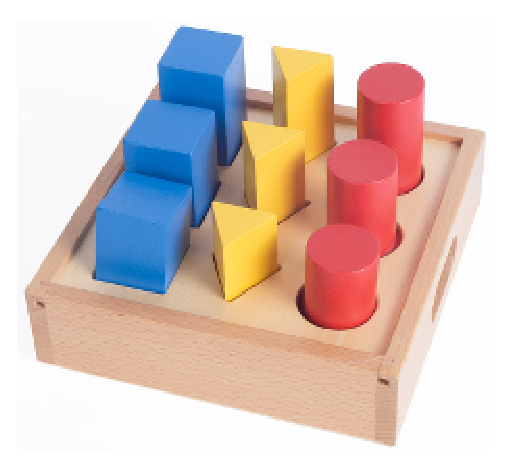
\includegraphics[width=3cm]{Geometrie_did/Images/Geo5_cours_boite_formes}
   \correction
   L'exemple typique de la boite à forme : dit-on : \og met le parallélépipède rectangle, le prisme et le cylindre dans les trous ? \fg. \\
   Non, on se contente de parler du carré, du triangle et du rond, ou dans le meilleur des cas du disque !
\end{exemple}

\smallskip

Au cours du {\bf cycle 2}, l’élève continue à travailler sur une géométrie de la perception, puis s'oriente progressivement en fin de cycle 2 et au {\bf cycle 3} vers une {\bf géométrie instrumentée} : la reconnaissance de la figure se fait à l'aide d'instruments. On passe d'un objet réel à un objet géométrique caractérisé grâce à  des propriétés liées aux instruments. Au {\bf cycle 4}, l’élève entre dans la {\bf géométrie axiomatique}, ou {\bf déductive} dans laquelle l'objet est défini par ses propriétés.

\begin{pspicture}(0,-10.5)(17,0.5)
   \psframe(0,0)(16,-1)
   \pspolygon(16,-1.5)(17,-0.5)(16,0.5)
   \psline(4,0)(4,-1)
   \psline(8,0)(8,-1)
   \psline(12,0)(12,-1)
   \rput(2,-0.5){cycle 1}
   \rput(6,-0.5){cycle 2}
   \rput(10,-0.5){cycle 3}
   \rput(14,-0.5){cycle 4}
   \pscustom[linestyle=none,fillstyle=gradient,gradangle=-90,
    gradbegin=yellow!50,gradend=white,
    gradmidpoint=0]{\psframe(0,-1)(8,-4)} % perspective
   \rput(4,-1.3){\bf géométrie perceptive}
   \psellipse[linewidth=0.7mm](1.2,-2.75)(0.4,0.6)
   \psellipse[linewidth=0.7mm](2,-2.75)(0.4,0.6)
   \psellipse[fillstyle=solid,fillcolor=blue](1.35,-2.75)(0.2,0.3)
   \psellipse[fillstyle=solid,fillcolor=blue](2.15,-2.75)(0.2,0.3)
   \psdots[linecolor=white](1.42,-2.75)(2.22,-2.75)
   \psarc[linewidth=1mm](1.2,-2.3){0.4}{45}{135}
   \psarc[linewidth=1mm](2,-2.3){0.4}{45}{135}
   \rput(4,-2.25){je vois}
   \rput(4,-2.65){un carré}
   \rput(4,-3.2){(objet)}
   \psframe[fillstyle=solid,fillcolor=B1,linecolor=B1](5.75,-1.75)(7.5,-3.5)
   \pscustom[linestyle=none,fillstyle=gradient,gradangle=-90,
    gradbegin=white,gradend=yellow!50,
    gradmidpoint=0.5]{\psframe(4,-4)(12,-7)} % instrument
   \rput(8,-4.4){\bf géométrie instrumentée}
   \rput(4.5,-6.5){\equerre{0}{0}{0}{0.7}}
   \psline[linewidth=1.3mm,linecolor=A1](5.2,-5)(5.7,-6.5)(5.7,-6.8)(5.7,-6.5)(6.2,-5)
   \pscircle[fillstyle=solid,fillcolor=A1](5.7,-6.4){0.18}
   \psline[linecolor=A1](5.15,-4.85)(5.7,-6.5)(6.25,-4.85)
   \rput(8,-5.1){j'utilise}
   \rput(8,-5.5){mon compas}
   \rput(8,-5.9){mon équerre}
   \rput(8,-6.3){(dessin)}
   \psframe[fillstyle=solid,fillcolor=B2!20](9.75,-4.75)(11.5,-6.5)
   \psdots[dotstyle=x,linewidth=0.8mm,linecolor=A1](10.625,-4.75)(10.625,-6.5)(9.75,-5.625)(11.5,-5.625)
   \psframe[linecolor=B1](9.75,-4.75)(10,-5)
   \psframe[linecolor=B1](9.75,-6.5)(10,-6.25)
   \psframe[linecolor=B1](11.5,-6.5)(11.25,-6.25)
   \psframe[linecolor=B1](11.5,-4.75)(11.25,-5)
   \pscustom[linestyle=none,fillstyle=gradient,gradangle=-90,
    gradbegin=white,gradend=yellow!50,
    gradmidpoint=0]{\psframe(8,-7)(16,-10)} % déduction
   \rput(12,-7.4){\bf géométrie déductive}
   \psframe(8.7,-9.6)(10,-8)
   \pscircle(8.85,-9.1){0.05}
   \pscircle(8.85,-8.5){0.05}
   \pslineByHand(9.2,-8.3)(9.8,-8.3)
   \pslineByHand(9.2,-8.55)(9.8,-8.55)
   \pslineByHand(9.2,-8.8)(9.8,-8.8)
   \psline[linecolor=red](9,-9.6)(9,-8)
   \rput(12,-8.2){j'utilise les}
   \rput(12,-8.7){propriétés}
   \rput(12,-9.2){(figure)}
   \pscustom[fillstyle=solid,fillcolor=B2!20]{\pslineByHand(13.75,-9.5)(13.75,-7.75)(15.5,-7.75)(15.5,-9.5)(13.75,-9.5)}
   \psline(13.75,-9.5)(15.5,-7.75)
   \psline(13.75,-7.75)(15.5,-9.5)
   \pspolygon[linecolor=B1](14.625,-8.625)(14.8,-8.45)(14.975,-8.625)(14.8,-8.8)
   \psdots[dotstyle=x,linewidth=0.8mm,linecolor=A1](14.1875,-8.1875)(14.1875,-9.0625)(15.0625,-8.1875)(15.0625,-9.0625)
   \psframe(0,0)(16,-1)
\end{pspicture}

Ce schéma synthétique est un peu réducteur et  il ne faut pas complètement cloisonner ces trois types de géométrie : en effet, la compétence \og raisonner \fg{} travaillée dès le cycle 2 implique un panachage des géométries, pour tracer un rectangle de dimensions données sur une feuille blanche, un élève de CM1 a besoin de se représenter l'objet, d'utiliser ses instruments, de connaître les propriétés caractéristiques du rectangle et de raisonner.


%%%%%%%%%%%%%%%%%
\section{Les outils de la géométrie}
%%%%%%%%%%%%%%%%%

Un instrument est formé de trois composantes : \\
   -- un artéfact, c’est-à-dire un objet matériel qui a été conçu dans un but déterminé ; \\
   -- une technique d’utilisation ; \\
   -- une théorie sous-jacente à l’usage de cet instrument.
   
À l'école primaire, les élèves ont recours à différentes règles (graduées ou non, de diverses tailles), à des gabarits, à l’équerre, au compas. Ils commenceront à utiliser le rapporteur uniquement au collège.

{\bf $\bullet$ La règle :} celle de l'élève est toujours graduée, ou pire (pour la géométrie), elle l'est des deux côtés. L'inconvénient principal de cette graduation visible est que l'élève aura tendance à vouloir mesurer, ce qui est une compétence des grandeurs et mesures mais pas de la géométrie (pure). Si on ne veut pas que la mesure soit utilisée, il suffit de mettre un scotch de couleur sur les graduations.
\begin{center}
   \begin{pspicture}(0,-0.5)(10,0)
      \psset{unit=0.5cm}
      \rput{180}(20,0){
      \rput{180}(20,.8){\psframe[linewidth=.8pt,framearc=0.5,fillstyle=solid,fillcolor=A3](-.4,1)(20.4,2)
      \psframe[fillstyle=solid,fillcolor=A3](-.4,-1)(20.4,1.2)
      \multido{\i=0+1}{21}{\psline(\i,1.7)(\i,2) \uput[d](\i,2){\tiny  \i}}
      \multido{\n=0.0+0.5}{41}{\psline[linewidth=.6pt](\n,1.8)(\n,2)}
      \multido{\n=0.0+0.1}{200}{\psline[linewidth=.4pt](\n,1.9)(\n,2)}}
      \psframe[fillstyle=solid,fillcolor=A4,linewidth=0pt](-.36,1.4)(20.36,1.77)
      }
   \end{pspicture}
\end{center} 
   
\begin{minipage}{12cm}
   {\bf $\bullet$ Le gabarit :} c' est un objet (papier, carton, métal) qui permet de vérifier la valeur d'un angle, ou de comparer deux angles, ou de construire un angle. Le plus classique est l'angle droit : n'importe quel coin d'une feuille rectangulaire est un gabarit d'angle droit. Son utilisation est indispensable avant l'introduction de l'équerre classique.
\end{minipage}
\begin{minipage}{4cm}
   \begin{pspicture}(-1,-0.5)(2,2)
      \pscustom[fillstyle=solid,fillcolor=brown!50]{\psline(2,0)(0,0)(0,2)\pscurve(0,2)(0.5,1.9)(1,1.1)(1.5,1)(2,0)}
   \end{pspicture}
\end{minipage}

\smallskip

\begin{minipage}{7.8cm}
   {\psset{unit=0.3}
      \begin{pspicture}(-3.5,0.5)(20,-11)
        \pspolygon[fillstyle=solid,fillcolor=A3](-1,0)(19,0)(-1,-10)
         \pspolygon[fillstyle=solid,fillcolor=white,linearc=0.2](1.5,-2.5)(9,-2.5)(1.5,-6)
         \multido{\i=0+1}{17}{\psline(\i,0)(\i,-0.5)\uput[d](\i,-0.2){\tiny  \i}}
         \multido{\r=0+0.5}{32}{\psline[linewidth=0.02](\r,0)(\r,-0.3)}
         \multido{\n=0+0.1}{160}{\psline[linewidth=0.01](\n,0)(\n,-0.2)}
      \end{pspicture}}
\end{minipage}
\begin{minipage}{8.5cm}
   {\bf $\bullet$ L'équerre :} c'est un gabarit d'angle droit, en général gradué mais comme pour le règle, les graduations sont inutiles pour la géométrie. L’équerre traditionnelle peut engendrer des représentations erronées relatives à l’angle droit (confusion avec le triangle, mauvaise utilisation en raison des trois angles présents sur une équerre).
\end{minipage}

\begin{minipage}{11cm}
   {\bf $\bullet$ Le compas :} permet de reporter des longueurs et de tracer des cercles (sans contrainte, à partir du centre et d'un point/de son rayon/de son diamètre). À l'origine, il s'agit d'un instrument qui est uniquement dédié aux reports de longueurs, notamment pour la navigation.
\end{minipage}
\hspace*{2cm}
\begin{minipage}{2cm}
   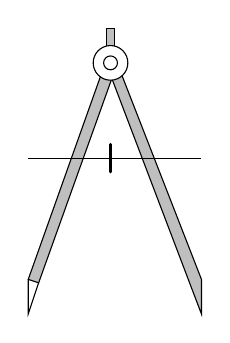
\begin{tikzpicture}[scale=2.2]
       \draw [fill=gray!50] (2.95,3.7) rectangle (3,3.95);
       \draw [fill=gray!50] (2.92,3.68) -- (2.5,2.5) -- (2.56,2.48) -- (2.99,3.68);
       \draw (3.5,2.5) -- (3.43,2.48);
       \draw [fill=gray!50] (3.04,3.68) -- (3.5,2.5) -- (3.5,2.3) -- (2.975,3.68);
       \draw (2.5,2.5) -- (2.5,2.3) -- (2.56,2.48) ;
       \draw [fill=white] (2.975,3.75) circle (0.1cm);
       \draw (2.975,3.75) circle (0.04cm);
       \draw (2.5,3.2) -- (3.5,3.2);
       \draw [line width = 1pt,line cap=round] (2.975,3.12) -- (2.975,3.28);
   \end{tikzpicture}
\end{minipage}

\smallskip

Le B.O. préconise de mobiliser des instruments variés lors des tracés : pochoirs, règles graduées et non graduées, bandes de papier avec un bord droit pour reporter des longueurs ou trouver un milieu, gabarits d’angle droit, équerres, compas. Certaines compétences de construction, comme tracer un segment d’une longueur donnée ou reporter la longueur d’un segment (CM1-CM2) sont menées conjointement avec les apprentissages du domaine \og grandeurs et mesures \fg{}. Cependant, ce travail doit d’abord pouvoir se faire sans règle graduée. \\
Voici un tableau récapitulant les liens entre les instruments et leurs propriétés géométriques :
\begin{center}
   \hautab{1.2}
   \begin{Ltableau}{\linewidth}{3}{m{2.8cm}|m{10.03cm}|m{2.7cm}}
       \hline
       Instrument & propriété géométrique & objet géométrique \\
       \hline
       Règle non graduée & alignement ; appartenance de points à une droite & droite \\
       \hline
       Règle graduée & distance entre deux points & segment \\
       \hline
       Gabarit & comparaison d'angles & angle \\
       \hline
       Equerre & perpendicularité ; parallélisme (en tant que double parallèle) ; distance entre un point et une droite & angle droit \\
       \hline
       Compas & égalité de longueurs ; report de longueurs & cercle \\
       \hline
   \end{Ltableau}
\end{center}


%%%%%%%%%%%%%%%%%%%%%%
\section{Explorer les formes à la maternelle}
%%%%%%%%%%%%%%%%%%%%%%

La connaissance des formes géométriques est une étape importante dans le développement de l’enfant. L'étude des formes en maternelle permet l'accès à la géométrie du cycle 2, participe à l'organisation de l'espace, à la perception du monde, joue un rôle dans l'apprentissage de l'écriture (tracés et identification des lettres).

De manière générale, la manipulation des objets peut être regroupée en trois types d'actions : \smallskip

{\hautab{1.2}
\begin{ltableau}{\linewidth}{3}
   \hline
   Catégoriser & Reproduire et assembler & Représenter \\
   \hline
   Consiste à considérer de manière équivalente de objets, des personnes ou des situations qui partagent des caractéristiques communes ; à réduire la complexité du monde en mettant de l’ordre dans ses connaissances en les subdivisant en catégories.
   &
   Les élèves disposent d’un objet et ils doivent en réaliser une copie. Il est possible de reproduire, avec des matériaux divers, un objet plus ou moins usuel, ou bien procéder à des aménagements ou à des compléments de fabrication.
   &
   Représenter un objet ou une situation spatiale, c’est l’évoquer à l’aide de procédés graphiques conventionnels (dessin à main levée, codage\dots) pour permettre une restitution proche de l’objet initial. \\
   \hline
   PS +++ \; MS +++ \; GS ++
   &
   PS ++ \; MS +++ \; GS +++
   &
   MS ++ \; GS +++ \\
   \hline
   $\bullet$ Différencier et classer des formes planes (lotos, dominos). \newline
   $\bullet$ Nommer des formes planes (bonhomme, portrait robot) .\newline
   $\bullet$ Reconnaître des formes planes (brochettes, kim).
   &
   $\bullet$ Reproduire un assemblage de formes planes (puzzles, tangrams). \newline
   $\bullet$ Reproduire des formes planes (géoplan, brochettes).
   &
  $\bullet$ Dessiner un assemblage de formes (drôles de bobines). \newline
  $\bullet$ Tracer des formes planes (pochoir, empruntes). \newline
  $\bullet$ Représenter un assemblage de formes planes (géoplan, bonhomme triangle). \\
   \hline
\end{ltableau}}

\begin{center}
   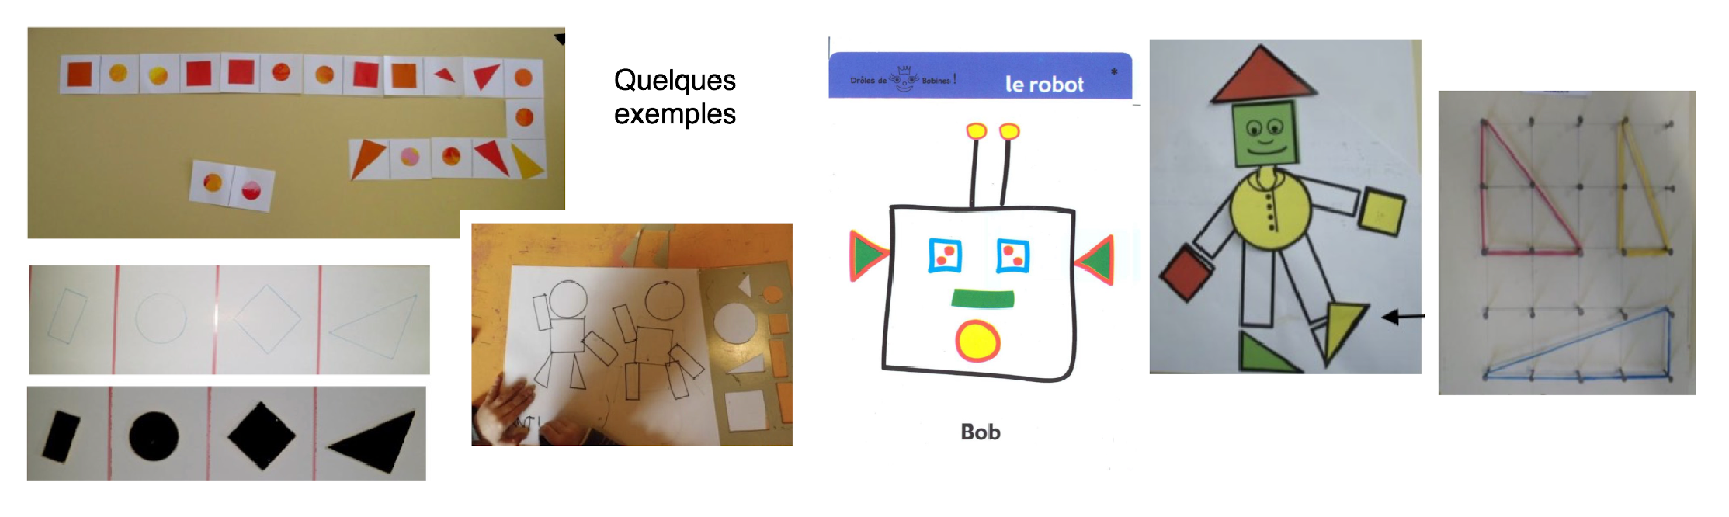
\includegraphics[width=16cm]{Geometrie_did/Images/Geo5_cours_formes_maternelle}
\end{center}


%%%%%%%%%%%%%%%%%%%%%%%%%%%%%%%
\section{Progressivité des apprentissages à l'école élémentaire}
%%%%%%%%%%%%%%%%%%%%%%%%%%%%%%%

-- Au {\bf CP} : 
\includegraphics[width=10mm]{Geometrie_did/Images/Geo5_cours_outils} la règle est utilisée comme outil de tracé de segments, et la règle graduée comme outil de mesure ou de report de longueur.  \\
   \hspace*{14mm} 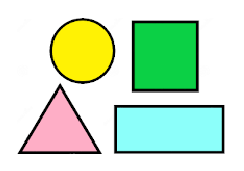
\includegraphics[width=10mm]{Geometrie_did/Images/Geo5_cours_formes} Les élèves reproduisent un carré, un rectangle, un triangle ou des assemblages de ces figures sur du papier quadrillé ou pointé, avec ou sans règle. \\
   \hspace*{14mm} 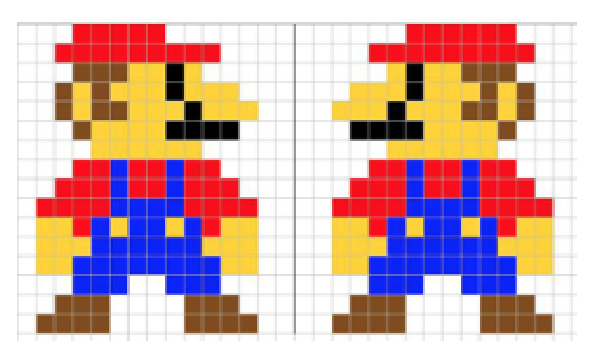
\includegraphics[width=10mm]{Geometrie_did/Images/Geo5_cours_symetrie} Il perçoivent des éléments symétriques dans leur environnement proche.  

-- Au {\bf CE1} : 
\includegraphics[width=10mm]{Geometrie_did/Images/Geo5_cours_outils} l'usage de la règle graduée est consolidé, ils découvrent l'équerre pour tracer ou reconnaître des angles droits et utilisent le compas pour tracer des cercles. \\
   \hspace*{16mm} 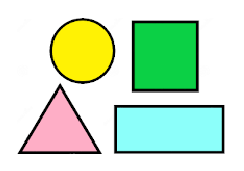
\includegraphics[width=10mm]{Geometrie_did/Images/Geo5_cours_formes} Les élèves consolident la reproduction d’un carré, d'un rectangle et d'un triangle sur un support uni, connaissant la longueur des côtés, à l'aide d'un règle et d'une équerre. Ils construisent des cercles sans contraintes, avec une ficelle ou un compas. \\
   \hspace*{16mm} 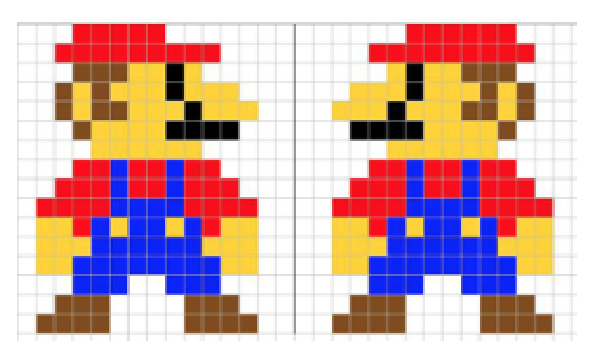
\includegraphics[width=10mm]{Geometrie_did/Images/Geo5_cours_symetrie} Ils reconnaissent si une figure présente un axe de symétrie, visuellement et/ou en utilisant du papier calque, des découpages, des pliages. 

-- Au {\bf CE2} : 
\includegraphics[width=10mm]{Geometrie_did/Images/Geo5_cours_outils} les élèves consolident l’utilisation de la règle graduée, de l’équerre et du compas. Ils abordent le report de longueur sur une droite déjà tracée, avec le compas. \\
   \hspace*{15mm} 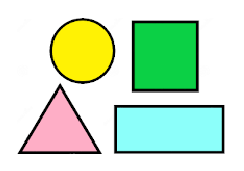
\includegraphics[width=10mm]{Geometrie_did/Images/Geo5_cours_formes} Ils consolident la construction de figures géométriques et construisent des cercles à partir du centre et du rayon ou du diamètre. \\
   \hspace*{15mm} 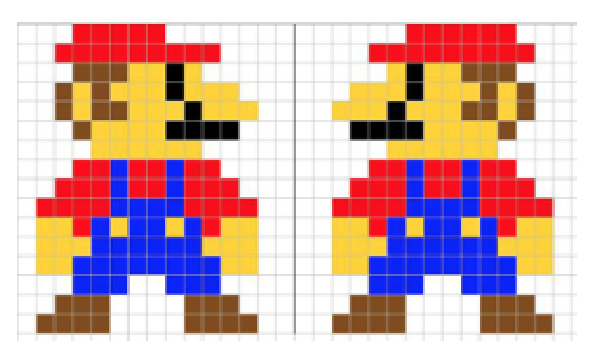
\includegraphics[width=10mm]{Geometrie_did/Images/Geo5_cours_symetrie} Ils complètent une figure pour qu'elle soit symétrique par rapport à un axe donné.

-- Au {\bf CM1} : 
\includegraphics[width=10mm]{Geometrie_did/Images/Geo5_cours_outils} les élèves utilisent la règle graduée ou non ainsi que des bandes de papier pour reporter des longueurs. Ils utilisent l’équerre pour repérer ou construire un angle droit, et d’autres gabarits d’angle ainsi que du papier calque. Ils utilisent le compas pour tracer un cercle, connaissant son centre et un point du cercle ou son centre et la longueur d’un rayon, ou bien pour reporter une longueur.  \\
   \hspace*{17mm} 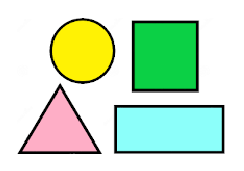
\includegraphics[width=10mm]{Geometrie_did/Images/Geo5_cours_formes} Ils consolident le vocabulaire du cycle 2 : côté, sommet, angle, angle droit, face, arête, milieu, droite, segment. Ils commencent à rencontrer la notation \og segment [AB] \fg{} mais cette notation n’est pas exigible ; pour les droites, on parle de la droite \og qui passe par les points A et B \fg, ou de \og la droite $d$ \fg. \\
   \hspace*{17mm} 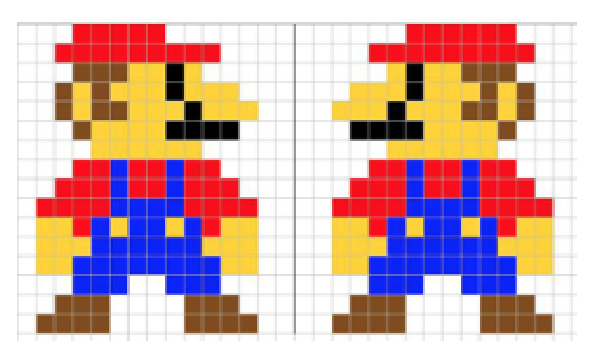
\includegraphics[width=10mm]{Geometrie_did/Images/Geo5_cours_symetrie} Ils reconnaissent qu’une figure admet un (ou plusieurs) axe de symétrie, visuellement et/ou par pliage ou en utilisant du papier calque. Ils complètent une figure par symétrie ou construisent le symétrique d’une figure donnée par rapport à un axe donné, par pliage et piquage ou en utilisant du papier calque.

-- Au {\bf CM2} : 
\includegraphics[width=10mm]{Geometrie_did/Images/Geo5_cours_outils} le travail sur les angles se poursuit, notamment sur des fractions simples de l’angle droit (demi ou tiers d'angle droit, angle plat comme somme de deux angles droits). \\
\hspace*{17mm} 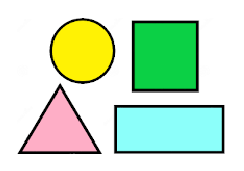
\includegraphics[width=10mm]{Geometrie_did/Images/Geo5_cours_formes} Les élèves commencent à rencontrer la notation \og droite (AB) \fg, et nomment les angles par leur sommet \og angle ($\widehat{A}$ \fg). \\
\hspace*{17mm} 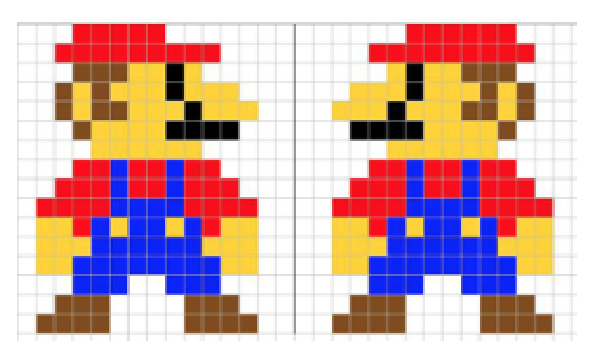
\includegraphics[width=10mm]{Geometrie_did/Images/Geo5_cours_symetrie} Ils observent que deux points sont symétriques par rapport à une droite donnée lorsque le segment qui les joint coupe cette droite perpendiculairement en son milieu et construisent, à l’équerre et à la règle graduée, le symétrique d’un point, d’un segment, d’une figure par rapport à une droite.


%%%%%%%%%%%%%%%%%%%%%%%%%%%%
%\subsection{Les supports}
%
%Pour tracer des figures, l'enseignant dispose de supports variés tels que le papier quadrillé, pointé ou uni. \\
%\begin{tabular}{ccc}
%\begin{pspicture}(-0.4,-0.5)(4.4,3.5)
%   \psgrid[subgriddiv=2,gridwidth=0.2mm,subgridwidth=0.2mm,subgridcolor=black,gridlabels=0](4,3)
%\end{pspicture}
%   &
%\begin{pspicture}(-0.4,-0.5)(4.4,3.5)
%   \psframe(0,0)(4,3)
%   \psgrid[subgriddiv=2,gridwidth=0.5mm,subgridwidth=0.5mm,griddots=1,subgriddots=1,subgridcolor=black,gridlabels=0](4,3)
%\end{pspicture}
%   &
%\begin{pspicture}(-0.4,-0.5)(4.4,3.5)
%   \psframe(0,0)(4,3)
%\end{pspicture}
%\end{tabular} \\
%Le papier quadrillé et le papier pointé servent à la reproduction de figures, au tracé de droites parallèles ou perpendiculaires, aux symétries. On peut, en utilisant les lignes du quadrillage ou le réseau pointé, construire certaines figures simples. L'utilisation du papier pointé à mailles carrées nécessite une bonne connaissance de l'utilisation du papier quadrillé : en effet, le papier pointé ne présente que les n\oe uds du quadrillage carré et il faut être capable de repérer qu'il s'agit d'un pavage de carrés. Un avantage du papier pointé est qu'il est moins chargé. \\
%
%\begin{minipage}{11cm}
%   On peut également utiliser un Géoplan :  une planche sur laquelle s’organisent des réseaux de clous, entre lesquels seront tendus des élastiques permettant de construire divers objets de géométrie plane (segments, triangles, contours polygonaux convexes ou non, figures géométriques\dots).
%\end{minipage}
%\qquad
%\begin{minipage}{5cm}
%   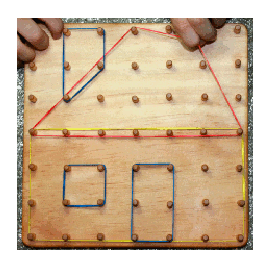
\includegraphics[width=3.5cm]{Geometrie_did/Images/Geo5_cours_geoplan}
%\end{minipage}


%%%%%%%%%%%%%
\section{Les figures planes}
%%%%%%%%%%%%%

{\renewcommand{\StringDOCUMENTATION}{Les figures à connaître}
\begin{documentation}
Au cycle 2, l'élève doit reconnaître et nommer les figures et objets usuels tels que :
\begin{itemize}
   \item carré, rectangle, triangle, triangle rectangle, polygone, cercle, disque ;
   \item côté, sommet, angle droit, rayon, centre, segment, milieu d’un segment, droite.
\end{itemize}
Au cycle 3, l'élève commence à utiliser les premières caractérisations des figures planes par leurs propriétés pour :
\begin{itemize}
   \item les triangles dont les triangles particuliers (rectangle, isocèle, équilatéral) ;
   \item les quadrilatères dont les quadrilatères particuliers (carré, rectangle, losange, approche du parallélogramme) ;
   \item le cercle comme ensemble de points situés à une distance donnée d'un point donné.
\end{itemize}
\end{documentation}}

\bigskip

Si l'entrée dans la géométrie des propriétés fait son apparition en grandes pompes en 6\up{e}, elle est déjà bien présente en début et milieu de cycle 3, ainsi qu'au cycle 2 avec la description à partir des côtés et des angles droits d'un carré, d'un rectangle et d'un triangle rectangle. 
\begin{center}
\begin{pspicture}(0,0)(15,9.5)
   \def\rec{\psframe[linecolor=B1](0,0)(0.3,0.3)}
   \rput(1.5,6.5){\small triangle quelconque} %%%%%
   \pspolygon(0,7)(3,7)(1,9)
   \rput(5.5,6.5){\small triangle rectangle} %%%%%
   \pspolygon(4,7)(7,7)(4,9)
   \rput(4,7)\rec
   \rput(9.5,6.5){\small triangle isocèle} %%%%%
   \pspolygon(8,7)(11,7)(9.5,8.5)
   \psdots[linecolor=A1,dotstyle=+,linewidth=0.8mm](8.75,7.75)(10.25,7.75)
   \rput(13.5,6.5){\small triangle équilatéral} %%%%%
   \pspolygon(12,7)(15,7)(13.5,9.6)
   \psdots[linecolor=A1,linewidth=0.5mm](13.5,7)(12.75,8.3)(14.25,8.3)
   \rput(1,3.5){carré} %%%%%
   \psframe(0,4)(2,6)
   \rput(0,4)\rec
   \rput(1.7,4)\rec
   \rput(0,5.7)\rec
   \rput(1.7,5.7)\rec
   \psdots[linecolor=A1,dotstyle=x,linewidth=0.8mm](1,4)(1,6)(0,5)(2,5)   
   \psframe(3,4)(6,6)
   \rput(4.5,3.5){rectangle} %%%%%
   \rput(3,4)\rec
   \rput(5.7,4)\rec
   \rput(3,5.7)\rec
   \rput(5.7,5.7)\rec
   \psdots[linecolor=A1,dotstyle=x,linewidth=0.8mm](3,5)(6,5)
   \psdots[linecolor=A1,dotstyle=|,linewidth=0.8mm](4.5,4)(4.5,6)
   \rput(8.75,3.5){losange} %%%%%
   \pspolygon(7,5)(8.75,4)(10.5,5)(8.75,6)
   \psdots[linecolor=A1,dotstyle=square*,linewidth=0.4mm](8,4.45)(9.5,4.45)(8,5.55)(9.5,5.55)
   \rput(13,3.5){parallélogramme} %%%%%
   \pspolygon(11.5,4)(14.5,4)(15,6)(12,6)
   \psdots[linecolor=A1,dotstyle=x,linewidth=0.8mm](11.75,5)(14.75,5)
   \psdots[linecolor=A1,dotstyle=|,linewidth=0.8mm](13,4)(13.5,6)
   \rput(2.5,0.5){polygone (à neuf côtés)} %%%%%
   \pspolygon(0,1)(2,1)(2.5,2)(4,1)(5,2.5)(4,3)(2,3)(1,2)(0,2.5)
   \rput(9,0.5){cercle} %%%%%
   \pscircle(9,2){1}
   \rput(13,1.5){disque} %%%%%
   \pscircle[fillstyle=solid,fillcolor=A3](13,1.5){1.5}
   \rput(13,1.5){disque} %%%%%
   \rput(9,2){+}
\end{pspicture}
\end{center}
À partir du CM2, on amène les élèves à dépasser la dimension perceptive et instrumentée pour raisonner sur les propriétés et les relations. Par exemple, l’usage de la règle et du compas pour tracer un triangle, connaissant la longueur de ses côtés, mobilise la connaissance des propriétés du triangle et de la définition du cercle. Les problèmes de reproduction de figures donnent l’occasion de dégager et travailler les propriétés et relations géométriques du programme. Le choix d’un support uni, quadrillé ou pointé et des instruments disponibles se fait suivant les objectifs. Les jeux du type portrait, Kim, etc., la construction de frises, pavages, rosaces peuvent contribuer à développer la connaissance des propriétés des figures du programme et du vocabulaire associé. \\ [-2mm]

L’initiation à l’utilisation de {\bf logiciels de géométrie dynamique} permettant de produire des figures se fait graduellement, en lien avec l’ensemble des activités, des connaissances et des compétences géométriques. 


%%%%%%%%%%
\section{La symétrie} 
%%%%%%%%%%

D'après le \og module sur la symétrie de l'université de Paris 5 dans le cadre de la TFM \fg{} : au cycle 2 et 3, les élèves mettent en place une première maîtrise de la symétrie. Ils passent peu à peu d’une reconnaissance perceptive de la symétrie axiale à l'utilisation de pliages, du miroir, du papier calque puis d’outils tels que règle, équerre, compas pour vérifier que deux figures sont symétriques ou ont un axe de symétrie pour finalement tracer la figure symétrique d’une figure donnée par rapport à un axe quelconque ou pour tracer la moitié symétrique d’une figure donnée par rapport à un axe. C'est en fin de cycle 3, en 6\up{e}, que l’étude systématique de la symétrie axiale se fera.


\subsection{Recherche d'un axe de symétrie} %%%


Pour conjecturer l'existence d'un axe, on repère : soit une sous-figure qui admet un axe de symétrie ; soit des éléments de la figure qui semblent symétriques (segments de même longueur, angles de même mesure) et on cherche alors à préciser leur axe de symétrie.

\begin{exemple}
   \psset{unit=1}
   \begin{pspicture}(-3,-0.5)(15,0.75)
      \psset{linewidth=0.1,unit=0.5}
      \psline(1.5,0)(0,0)(0,2)(1.5,2)%B
      \psline(0,1)(1.5,1)
      \psarc(1.5,0.5){0.5}{270}{90}
      \psarc(1.5,1.5){0.5}{270}{90}      
      \psline(3,0)(5,0)%I
      \psline(3,2)(5,2)
      \psline(4,0)(4,2)     
      \psline(6,2)(8,2)%J
      \psline(7,0.5)(7,2)
      \psarc(6.5,0.5){0.5}{180}{360}
      \psline(6,0.5)(6,1)
      \pscircle(10,1){1}%O
      \psline(12,1)(12,2)
      \psline(14,1)(14,2)
      \psarc(13,1){1}{180}{360}
      \psline(15,0)(17,2)%X
      \psline(15,2)(17,0)      
      \psset{linewidth=0.05,linecolor=B2,linestyle=dashed}
      \psline(-0.5,1)(2.5,1)
      \psset{linewidth=0.05,linecolor=A1,linestyle=dashed}
      \psline(2.5,1)(5.5,1)
      \psline(4,-0.5)(4,2.5)
      \psset{linewidth=0.05,linecolor=J1,linestyle=dashed}
      \psline(8.5,1)(11.5,1)
      \psline(10,-0.5)(10,2.5)
      \psline(8.5,-0.5)(11.5,2.5)
      \psline(8.5,2.5)(11.5,-0.5)
      \psline(9.5,-0.5)(10.5,2.5)
      \psline(9.5,2.5)(10.5,-0.5)
      \psline(8.5,0)(11.5,2)
      \psline(8.5,0.5)(11.5,1.5)
      \psline(8.5,2)(11.5,0)
      \psline(8.5,1.5)(11.5,0.5)
      \psset{linewidth=0.05,linecolor=gray,linestyle=dashed}
      \psline(13,-0.5)(13,2.5)
      \psset{linewidth=0.05,linecolor=G1,linestyle=dashed}
      \psline(14.5,1)(17.5,1)
      \psline(16,-0.5)(16,2.5)
      \psline(14.5,-0.5)(17.5,2.5)
      \psline(14.5,2.5)(17.5,-0.5)
   \end{pspicture}
\end{exemple}

{\renewcommand{\StringDOCUMENTATION}{Pour vérifier que l'axe conjecturé est bien un axe de symétrie de la figure, on peut}
\begin{documentation}
   \begin{itemize}
      \item effectuer le pliage et vérifier que les deux parties de la figure situées dans les demi-plans définis par la droite se superposent ;
      \item utiliser du matériel pédagogique comme le géomiroir, qui laisse passer le regard tout en réfléchissant l'image de la figure ;
      \item utiliser du papier calque pour vérifier que les deux figures se correspondent ;
      \item tracer mentalement le symétrique de la figure et repérer s'il fait partie de la figure. \\ [-8mm]
   \end{itemize}
\end{documentation}}

\bigskip

Difficultés et erreurs concernant la recherche d'axe(s) de symétrie : \\
{\bf $\bullet$ Orientation de l'axe} : les élèves privilégient les axes verticaux ou horizontaux, dans la mesure où ils le sont souvent dans leur contexte social et scolaire. Si une figure possède des axes de symétrie ni horizontaux ni verticaux, certains élèves ne les verront pas. \\
{\bf $\bullet$ Nombre d'axes de symétrie} : si plusieurs axes de symétrie existent, l'élève, après en avoir trouvé un, peut considérer que sa tâche est terminée et donc ne pas en chercher d'autres. \\
{\bf $\bullet$ Familiarité que l'élève a avec la figure} : le figue est-elle une image connue par l'élève ? Si oui, il déterminera plus facilement le ou les axes de symétrie. \\
{\bf $\bullet$ Théorème en acte} : beaucoup d'élèves s'appuient sur le théorème-élève suivant : \og un axe de symétrie d'une figure passe par le milieu de cette figure \fg, sans penser que la réciproque est fausse. \\
{\bf $\bullet$ Figures élémentaires} : dans le cas où la figure est composée de figures élémentaires facilement repérables et possédant chacun un axe de symétrie, les élèves ont tendance à assimiler ces axes comme ceux de la figure complète.
   
\begin{exemple*1}
   En pointillé les axes que certains élèves ne reconnaissent pas, en gras ceux qu'ils pensent reconnaître. \\
   {\psset{unit=0.5}
   \begin{pspicture}(-1.5,1)(8,4)
      \rotatebox{45}{
         \pspolygon(0,1)(2,0)(4,1)(2,2)
         \psline[linecolor=A1,linestyle=dashed](-0.5,1)(4.5,1)
         \psline[linecolor=A1,linestyle=dashed](2,-0.5)(2,2.5)}
      \pspolygon(4.5,1)(7.5,1)(6,3.6)
      \psline[linecolor=A1](6,0.5)(6,4)
      \psline[linecolor=A1,linestyle=dashed](4.5,1)(7,2.42)
      \psline[linecolor=A1,linestyle=dashed](7.5,1)(5,2.42)
   \end{pspicture}
   \begin{pspicture}(-1.75,0)(12,2.5)
      \psframe(0,0)(4,2)
      \psline[linecolor=A1,linewidth=0.7mm](-0.5,-0.25)(4.5,2.25)
      \psline[linecolor=A1](2,-0.5)(2,2.5)
      \psline[linecolor=A1](-0.5,1)(4.5,1)
      \pspolygon(6,0)(10,0)(11,2)(7,2)
      \psline[linecolor=A1,linewidth=0.7mm](8.5,-0.5)(8.5,2.5)
   \end{pspicture}
   \begin{pspicture}(0,0)(4,2.5)
      \psframe(0,0)(3,2)
      \pscircle(4,1){1.4}
      \rput(4,1){$\times$}
      \psline[linecolor=A1,linewidth=0.7mm](4,-0.75)(4,2.75)
      \psline[linecolor=A1,linewidth=0.7mm](1.5,-0.5)(1.5,2.5)
      \psline[linecolor=A1,linestyle=dashed](-0.5,1)(5.8,1)
   \end{pspicture}}
\end{exemple*1}


\subsection{Tracer le symétrique d'une figure par rapport à un axe} %%%

Il est nécessaire que les élèves aient travaillé avec le pliage et aient utilisé au moins un miroir afin qu’ils aient une bonne représentation de ce qu’est la symétrie axiale. Si l’on s’engage trop rapidement dans un travail sur les tracés sans ces prérequis, les élèves risquent de produire des figures erronées et ne pas comprendre leurs erreurs. Il faut aussi que les élèves soient capables de reconnaître si des figures sont superposables, qu’ils aient des notions concernant la perpendicularité : reconnaître que deux droites sont perpendiculaires,  tracer une droite perpendiculaire à une autre quelle que soit sa direction. Les situations doivent conduire les élèves à utiliser des techniques qui évoluent en fonction des supports et des instruments choisis ; par exemple, passer du pliage ou de l’utilisation de papier calque à la construction du symétrique d’un point par rapport à une droite à l’équerre et à la droite graduée.
{\renewcommand{\StringDOCUMENTATION}{Les procédures de tracé du symétrique d'une figure}
\begin{documentation}
\begin{itemize}
   \item {\bf Par pliage} : plier la feuille suivant l'axe de symétrie, puis décalquer la figure par transparence. Aucune connaissance mathématique n'est à connaître ici.
   \item {\bf Avec un papier calque} : décalquer la figure de départ ainsi que l'axe, retourner le papier calque et replacer ce papier sur la feuille en plaçant correctement l'axe, et enfin repasser le crayon sur la figure afin qu'elle laisse une emprunte sur la feuille.
   \item {\bf Avec une équerre et une règle graduée} : tracer la perpendiculaire à l'axe de symétrie passant par le point dont on veut déterminer le symétrique à l'aide de son équerre, puis avec la règle, reporter sur cette perpendiculaire la distance du point à l'axe. \\
   {\psset{unit=0.55}
   \begin{pspicture}(-2,0)(5,3.75)
      \pstGeonode[PointSymbol=none,PointName=none](1,3){A}(3,0){B}
      \pstGeonode[PointName=none,linewidth=0.3mm](3,3){C}
      \pstLineAB{A}{B}       
   \end{pspicture}
   \qquad
   \begin{pspicture}(-1,0)(5,3.75)
      \pstGeonode[PointSymbol=none,PointName=none](1,3){A}(3,0){B}
      \pstGeonode[PointName=none,linewidth=0.3mm](3,3){C}
      \pstLineAB{A}{B}  
      \pstOrtSym[PointSymbol=none,PointName=none]{A}{B}{C}[D]           
      \pstLineAB[linecolor=A1,linewidth=0.05,nodesepB=-1]{C}{D} 
      \equerre{1.1}{1.38}{-57}{1.5}
   \end{pspicture}
   \qquad
   \begin{pspicture}(-1,0)(4,3.75)
      \pstGeonode[PointSymbol=none,PointName=none](1,3){A}(3,0){B}
      \pstGeonode[PointName=none,linewidth=0.3mm](3,3){C}
      \pstLineAB{A}{B}  
      \pstOrtSym[PointName=none,linewidth=0.3mm]{A}{B}{C}[D]           
      \pstLineAB[linecolor=A1,linewidth=0.05,nodesepB=-1]{C}{D} 
      \psarc[linestyle=dashed,linecolor=B2](1.62,2.05){1.67}{20}{50}
      \psarc[linestyle=dashed,linecolor=B2](1.62,2.05){1.67}{200}{230}
      \rput(2.3,2.53){$\backslash\backslash$}
      \rput(1,1.65){$\backslash\backslash$}
      \pstMiddleAB[PointSymbol=none,PointName=none]{C}{D}{I}
      \pstRightAngle[linecolor=J1]{C}{I}{B}
   \end{pspicture}}
   \item {\bf Sur papier quadrillé : } placer le symétrique de chacun des points en s'aidant du quadrillage, puis relier ces points entre eux, ou, placer un premier point symétrique, puis construire la figure symétrique inversée point par point. \\ [-8mm]
\end{itemize}
\end{documentation}}

\bigskip

Difficultés et erreurs concernant la construction de la figure symétrique : \\
{\bf $\bullet$ Mauvais dénombrement des carreaux :} l'élève se trompe dans le dénombrement des carreaux lors de la construction du symétrique d'un point. Il ne s'agit pas d'une erreur de compréhension. \\
{\bf $\bullet$ Erreur dans l'ordre du tracé :} lorsque le nombre de sommets d'un polygone dont il faut tracer le symétrique est important, l'élève trace le symétrique de tous les points puis il se trompe dans l'ordre de jonction de ces points. \\
{\bf $\bullet$ Construction du translaté :} consiste à construire le symétrique d'un point correctement puis à placer l'image de la figure en la translatant. Cette erreur est d'autant plus présente si la figure est elle même presque symétrique. \\
{\bf $\bullet$ Axe de symétrie oblique :} dans le cas d'un axe ne suivant pas les lignes du quadrillage, l'élève va néanmoins suivre les lignes du quadrillage comme si l'axe était horizontal ou vertical ou à la manière d'une symétrie centrale.

\smallskip
  
\begin{exemple*1}
   {\psset{unit=0.6}
   \begin{pspicture}(-1.5,0)(9,4)
      \psgrid[griddots=8,subgriddiv=0, gridlabels=0pt,gridcolor=gray](-1,-1)(9,4)
      \psframe(0,0)(3,2)
      \pspolygon(0,2)(3,2)(2,3)
      \psline(1,0)(1,1)(2,1)(2,0)
      \psline[linecolor=A1,linewidth=0.5mm](4,-1)(4,4)
      \psframe[linecolor=B2](5,0)(8,2)
      \pspolygon[linecolor=B2](5,2)(8,2)(7,3)
      \psline[linecolor=B2](6,0)(6,1)(7,1)(7,0)
   \end{pspicture}
   \begin{pspicture}(-2.5,0)(9,2.8)
      \psgrid[griddots=8,subgriddiv=0, gridlabels=0pt,gridcolor=gray](-1,-1)(9,4)
      \psline(0,1)(3,1)(3,3)
      \psline(2,1)(2,2)
      \psline[linecolor=A1,linewidth=0.5mm](2,-1)(6,3)
      \psline[linecolor=B2](8,1)(5,1)(5,-1)
      \psline[linecolor=B2](6,1)(6,0)
   \end{pspicture}}
   \end{exemple*1}


%%%%%%%%%%%%%%%%%%%%%%%%%%%
\section{Programmes de construction} %
%%%%%%%%%%%%%%%%%%%%%%%%%%%

Dans le B.O., on trouve le vocabulaire suivant : {\bf décrire, reproduire, construire} des objets géométriques. On peut schématiser les trois types d'activités par les schémas suivants. La difficulté de ces types de tâches est croissante. 
\begin{center}
\begin{tabular}{C{5}C{5}C{5}}
   Reproduire & Construire & Décrire \\
   \begin{pspicture}(0,0.3)(4.5,1.9)
      \Figure
      \psline[linewidth=3pt,arrowlength=1.25]{->}(2.2,1.2)(2.7,1.25)
      \rput(2.7,0){\Figure}
   \end{pspicture}
   &
   \begin{pspicture}(0,0.3)(4.5,1.9)
      \Texte
      \psline[linewidth=3pt,arrowlength=1]{->}(2.2,1.25)(2.7,1.25)
      \rput(2.7,0){\Figure}
   \end{pspicture}
   &
   \begin{pspicture}(0,0.3)(4.5,1.9)
      \Figure
      \psline[linewidth=3pt,arrowlength=1]{->}(2.2,1.25)(2.7,1.25)
     \rput(2.7,0){\Texte}
   \end{pspicture}
\end{tabular}
\end{center}

\textbf{$\bullet$ La reproduction} d'une figure géométrique est la construction une figure géométrique à partir d’un modèle fourni avec les mêmes dimensions ou en respectant une certaine échelle.

{\renewcommand{\StringDOCUMENTATION}{Difficultés liées aux tâches de reproduction}
\begin{documentation}
\begin{itemize}
   \item Repérage des figures de base d'une figure complexe : configurations non reconnues, figures non prototypiques, difficultés à isoler les figures de base des autres éléments\dots 
   \item Identification des relations entre les figures élémentaires.
   \item Chronologie du tracé.
   \item Exécution de tracés géométriques. \\ [-8mm]
\end{itemize}
\end{documentation}}

\bigskip

%%%%%%%%%%%%%%%%%%
\textbf{$\bullet$ La construction} consiste à réaliser une figure géométrique plane à partir d’un programme de construction, un texte descriptif, une figure à main levée, etc.

{\renewcommand{\StringDOCUMENTATION}{Difficultés liées aux tâches construction}
\begin{documentation}
\begin{itemize}
   \item Vocabulaire géométrique plus ou moins acquis.
   \item Mobilisation d'images mentales anticipatrices.
   \item Manipulation des instruments de tracé (difficultés psychomotrices). \\ [-8mm]
\end{itemize}
\end{documentation}}

\bigskip

%%%%%%%%%%%%%%%%%%
\textbf{$\bullet$ La description} d'une figure revient à élaborer un message en utilisant le vocabulaire géométrique approprié et en s’appuyant sur les caractéristiques d’une figure géométrique pour en permettre sa représentation ou son identification.

{\renewcommand{\StringDOCUMENTATION}{Difficultés liées aux tâches de description}
\begin{documentation}
 \begin{itemize}
    \item Au niveau du vocabulaire : l'élève ne connaît pas certains mots mathématiques, il les confond, il utilise certains mots mots du langage courant qui n'ont pas de sens en maths.
   \item Utilisation insuffisamment précise du vocabulaire.
   \item Manque de connaissance des propriétés caractérisant les figures de base. \\ [-8mm]
\end{itemize}
\end{documentation}}

\ \\

La pratique de ces tâches tout au long du cycle 3 conduit à prévoir des éléments de différenciation dépendant des besoins des élèves reposant sur des choix et des évolutions concernant : \\
-- le support de construction des figures : papier pointé, quadrillé, uni, logiciel de géométrie/programmation\dots ; \\
-- la nature des figures, des éléments qui la composent ; \\
-- les éléments directement visibles (analyse immédiate) ou non tracés (à trouver) pour reproduire (alignement, prolongement, milieu, angles droits, parallèles\dots) ; \\
-- les contraintes pour la reproduction : support, tracé à main levée avec des codages ou tracé avec des instruments, présence ou non d’une amorce à compléter, instruments autorisés, échelle\dots


%%%%%%%%%%%%%%%%%%%%%%%%%%%%%
%%%%%%%%%%%%%%%%%%%%%%%%%%%%%
\activites

\textcolor{G1}{Proposition n°4 : Figures géométriques de \og {\it Préparation CRPE 2022 COPIRELEM} \fg, ARPEME, page 223.} \bigskip

{\bf\uline{Consigne candidat}} : Vous êtes enseignant(e) en CE2, et vous souhaitez mettre en œuvre une séquence visant à apprendre aux élèves à \og {\it Reproduire sur papier quadrillé ou uni de figures planes (éventuellement à partir d’éléments déjà fournis de la figure à reproduire qu’il s’agit alors de compléter […] Décrire à partir des côtés et des angles droits, un carré, un rectangle, un triangle rectangle} \fg. \bigskip
Vous présenterez une séance de cette séquence construite à partir des énoncés de problèmes proposés en annexe 1, en incluant une phase de synthèse des apprentissages visés. \\
Pour anticiper son déroulement, vous pourrez prendre appui sur les photographies regroupées dans l’annexe 2. \\
Les annexes 3 et 4 pourront vous être utiles pour préciser et justifier les enjeux de la séance que vous proposerez et les variables didactiques mises en jeu dans les deux problèmes proposés. \bigskip

{\bf\uline{Connaissance ou compétence visée}} : Reconnaître, nommer, décrire, reproduire, construire quelques figures géométriques. \bigskip

{\bf\uline{Contexte de la séance d'enseignement}} : \\
   \hspace*{5mm} -- cycle d'enseignement : cycle 2 ; \\
   \hspace*{5mm} -- niveau de la classe : CE2 ; \\
   \hspace*{5mm} -- domaine : Espace et géométrie ; \\ [2mm]

{\bf\uline{Documents fournis au candidat}} : \bigskip

{\bf\uline{Document 1}} : Extraits {\it Programme d’enseignement du cycle des apprentissages fondamentaux (cycle 2}), en vigueur a la rentrée 2020. Ministère de l'Education nationale de la Jeunesse et des Sports. \bigskip

\begin{center}
   \begin{minipage}{16cm}
      \textsf{\textcolor{teal}{\bf\large Espace et Géométrie} \\
         Au cycle 2, les élèves acquièrent à la fois des connaissances spatiales comme l’orientation et le repérage dans l’espace et des connaissances géométriques sur les solides et sur les figures planes. Apprendre à se repérer et se déplacer dans l’espace se fait en lien étroit avec le travail dans \og Questionner le monde \fg{} et \og Éducation physique et sportive \fg. Les connaissances géométriques contribuent à la construction, tout au long de la scolarité obligatoire, des concepts fondamentaux d’alignement, de distance, d’égalité de longueurs, de parallélisme, de perpendicularité, de symétrie. \\
         Les compétences et connaissances attendues en fin de cycle se construisent à partir de manipulations et de problèmes concrets, qui s’enrichissent tout au long du cycle en jouant sur les outils et les supports à disposition, et en relation avec les activités mettant en jeu les grandeurs géométriques et leur mesure. \\
         Dans la suite du travail commencé à l’école maternelle, l’acquisition de connaissances spatiales s’appuie sur des problèmes visant à localiser des objets ou à décrire ou produire des déplacements dans l’espace réel. L’oral tient encore une grande place dans l’ensemble du cycle mais les représentations symboliques se développent et l’espace réel est progressivement mis en relation avec des représentations géométriques. La connaissance des solides se développe à travers des activités de tri, d’assemblages et de fabrications d’objets. Les notions de géométrie plane et les connaissances sur les figures usuelles s’acquièrent à partir de manipulations et de résolutions de problèmes (reproduction de figures, activités de tri et de classement, description de figures, reconnaissance de figures à partir de leur description, tracés en suivant un programme de construction simple). La reproduction de figures diverses, simples et composées est une source importante de problèmes de géométrie dont on peut faire varier la difficulté en fonction des figures à reproduire et des instruments disponibles. Les concepts généraux de géométrie (droites, points, segments, angles droits) sont présentés à partir de tels problèmes. \\
         En géométrie comme ailleurs, il est particulièrement important que les professeurs utilisent un langage précis et adapté et introduisent le vocabulaire approprié au cours des manipulations et situations d’action où il prend sens pour les élèves, et que ceux-ci soient progressivement encouragés à l’utiliser.}
   \end{minipage}
\end{center}

\begin{center}
   \begin{minipage}{16cm}
      \textsf{   
         \begin{tabular}{p{15cm}}
            \cellcolor{A3!50}{{\bf Attendus de fin de cycle} \newline
               -- (Se) repérer et (se) déplacer en utilisant des repères et des représentations. \newline
               -- Reconnaître, nommer, décrire, reproduire quelques solides. \newline
               -- Reconnaître, nommer, décrire, reproduire, construire quelques figures géométriques. \newline
               - Reconnaître et utiliser les notions d’alignement, d’angle droit, d’égalité de longueurs, de milieu, de symétrie.} \\
         \end{tabular} \\ [3mm]
         \begin{tabular}{|p{14.9cm}|}
            \hline
            \textcolor{teal}{\bf Reconnaître, nommer, décrire, reproduire, construire quelques figures géométriques Reconnaître et utiliser les notions d’alignement, d’angle droit, d’égalité de longueurs, de milieu, de symétrie} \\
            \hline
            -- Décrire, reproduire sur papier quadrillé ou uni des figures ou des assemblages de figures planes ({\it éventuellement à partir d’éléments déjà fournis de la figure à reproduire qu’il s’agit alors de compléter}). \newline
            -- Utiliser la règle, le compas ou l’équerre comme instruments de tracé. \newline
            -- Reconnaître, nommer les figures usuelles : carré, rectangle, triangle, triangle rectangle, polygone, cercle, disque. \newline
            -- Décrire à partir des côtés et des angles droits, un carré, un rectangle, un triangle rectangle. Les construire sur un support uni connaissant la longueur des côtés. \newline
            -- Construire un cercle connaissant son centre et un point, ou son centre et son rayon : \newline
            \hspace*{5mm} o vocabulaire approprié pour décrire les figures planes usuelles : \newline
            \hspace*{10mm} $\square$ carré, rectangle, triangle, triangle rectangle, polygone, côté, sommet, angle droit ; \newline
            \hspace*{10mm} $\square$ cercle, disque, rayon, centre ; \newline
            \hspace*{10mm} $\square$ segment, milieu d’un segment, droite. \newline
            \hspace*{5mm} o propriété des angles et égalités de longueur des côtés pour les carrés et les rectangles ; \newline
            \hspace*{5mm} o lien entre propriétés géométriques et instruments de tracé : \newline
            \hspace*{10mm} $\square$ droite, alignement et règle non graduée ; \newline
            \hspace*{10mm} $\square$ angle droit et équerre ; \newline
            \hspace*{10mm} $\square$ cercle et compas. \\
            \hline 
            -- Utiliser la règle (non graduée) pour repérer et produire des alignements. \newline
            -- Repérer et produire des angles droits à l'aide d’un gabarit, d'une équerre. \newline
            -- Reporter une longueur sur une droite déjà tracée, en utilisant une bande de papier avec un bord droit ou la règle graduée ou le compas (en fin de cycle). \newline
            -- Repérer ou trouver le milieu d’un segment, en utilisant une bande de papier avec un bord droit ou la règle graduée : \newline
            \hspace*{5mm} o alignement de points et de segments ; \newline
            \hspace*{5mm} o angle droit ; \newline
            \hspace*{5mm} o égalité de longueurs ; \newline
            \hspace*{5mm} o milieu d’un segment. \\
            \hline
            -- Reconnaître si une figure présente un axe de symétrie (à trouver), visuellement et/ou en utilisant du papier calque, des découpages, des pliages. \newline
            -- Reconnaître dans son environnement des situations modélisables par la symétrie (papillons, bâtiments, etc.). \newline
            -- Compléter une figure pour qu'elle soit symétrique par rapport à un axe donné : \newline
            \hspace*{5mm} o symétrie axiale ; \newline
            \hspace*{5mm} o une figure décalquée puis retournée qui coïncide avec la figure initiale est symétrique : elle a un axe de symétrie (à trouver) ; \newline
            \hspace*{5mm} o une figure symétrique pliée sur son axe de symétrie, se partage en deux parties qui coïncident exactement. \\
            \hline
      \end{tabular}
   }
   \end{minipage}
\end{center}

\pagebreak


{\bf\uline{Document 2}} : Extrait de Mathé A.-C., Barrier T., Perrin-Glorian M.-J. (2020). {\it Enseigner la géométrie élémentaire. Enjeux, ruptures et continuités}. Éditions Academia – L’Harmattan, pp. 94-95.
\begin{center}
   \begin{minipage}{16cm}
      \textsf{[…] la géométrie élémentaire recouvre en réalité au moins deux types de pratiques géométriques aux fondements épistémologiques différents mais tous deux cohérents, que nous avons appelés géométrie physique et géométrie théorique. La géométrie physique, à laquelle se réfère principalement l’enseignement primaire, se propose de résoudre des problèmes portant sur des objets matériels, qui peuvent être graphiques, à l’aide d’instruments matériels. La géométrie théorique avec pour modèle la géométrie euclidienne, à laquelle se réfère principalement l’enseignement secondaire, prend pour objet d’étude des figures théoriques et comme moyen de validation le raisonnement hypothético-déductif. La rupture entre ces deux manières de faire de la géométrie se manifeste dans la nature des problèmes posés et des objets étudiés, et surtout dans les modes de validation pratiqués. Cependant, ces géométries entretiennent des liens étroits, que l’on peut utiliser dans l’enseignement, pour autant que l’on dégage les enjeux d’apprentissage conceptuels du travail instrumenté sur les figures matérielles. C’est ce que nous efforçons de faire dans ce que nous avons appelé la géométrie des tracés. \\
Notre approche vise à penser un enseignement de la géométrie continu et cohérent, du début du primaire jusqu’au milieu du secondaire, en nous attachant à deux idées fondamentales. La première réside dans la nécessité de viser la construction progressive d’un rapport géométrique aux figures matérielles. D’abord objets d’étude pris pour eux-mêmes, les figures deviennent progressivement représentants d’objets plus généraux et abstraits. La géométrie du secondaire les élaborera en objets théoriques en les incluant dans un cadre axiomatique. Par ailleurs, interpréter géométriquement une figure matérielle suppose une capacité à mobiliser une manière de voir et d’analyser les figures, spécifique à la géométrie, dans un mouvement de déconstruction et reconstruction dimensionnelle. Cette visée constitue pour nous un enjeu fondamental de la géométrie de l’école primaire (et du début du secondaire). \\
La seconde idée porte sur le rôle que peut jouer le traitement instrumenté de figures matérielles dans le processus de conceptualisation en géométrie. Au-delà d’un usage précis des instruments, l’enseignement de la géométrie au primaire et au début du secondaire vise la conceptualisation d’objets et de relations géométriques. Cette conceptualisation repose sur un usage juste plutôt que précis des instruments, c’est-à-dire en lien avec les propriétés qu’ils permettent de représenter, ce que nous avons appelé un usage géométrique des instruments. Faire évoluer la capacité d’analyse des figures en jouant sur les instruments à disposition conduit à l’élaboration de schèmes d’utilisation de ces instruments qui, de manière articulée avec un travail langagier, viennent soutenir la conceptualisation géométrique. Notre approche vise ainsi la coordination de trois dimensions majeures : la mobilité du regard sur les figures matérielles, le double rôle des instruments (matériels et théoriques) et le langage géométrique. Les situations de reproduction de figure à l’aide d’instruments et les situations de formulation et de validation auxquelles elles donnent lieu sont un moyen d’y parvenir, par un jeu sur les variables didactiques.
      }
   \end{minipage}
\end{center}

\bigskip

{\bf\uline{Document 3}} : Documents de travail pour les élèves, avec une photographie du matériel mis à leur disposition.

\begin{center}
   \fbox{\begin{minipage}{14cm}
      \textsf{
         \begin{pspicture}(1,1.2)(14,5.7)
            \rput(7.5,5.4){\bf Géométrie. Tracer un carré, connaître ses propriétés}
            \rput(4,4.9){\underline{Modèle}}
            \rput{60}(5,1.3){\psframe(0,0)(2.3,2.3)}
            \rput(12,4.9){\underline{Gabarit fourni}}
            \rput(12,3){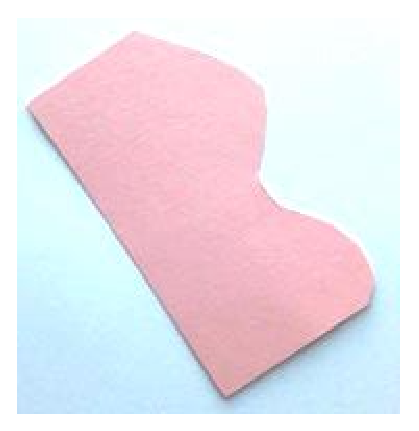
\includegraphics[width=3cm]{Geometrie_did/Images/Geo5_crpe_gabarit_angle}}
         \end{pspicture} \\
         1) Reproduis le carré en utilisant les instruments suivants : \\
            \hspace*{1cm} -- gabarit de carré \og grignoté \fg{} {\it (le gabarit dans l’image ci-dessus)} \hspace*{1cm} -- crayon. \\
         2) Après avoir effectué ce tracé, quelle(s) propriété(s) du carré as-tu mise(s) en évidence ?}
   \end{minipage}}
\end{center}

\begin{center}
   \fbox{\begin{minipage}{14cm}
      \textsf{
         \begin{pspicture}(1,1.3)(14,5)
            \rput(4,4.8){\underline{Modèle}}
            \rput{60}(5,1.3){\psframe(0,0)(2.3,2.3)}
            \rput(12,4.8){\underline{Gabarit fourni}}
            \rput(12,3){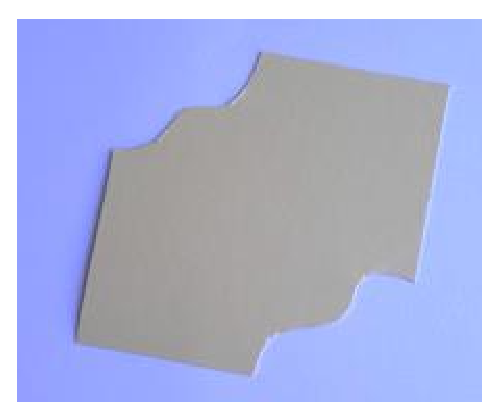
\includegraphics[width=3cm]{Geometrie_did/Images/Geo5_crpe_gabarit_angle_bis}}
         \end{pspicture} \\
         1) Reproduis le carré en utilisant les instruments suivants : \\
            \hspace*{1cm} -- gabarit de carré \og grignoté \fg{} {\it (le gabarit dans l’image ci-dessus)} \hspace*{1cm} -- crayon. \\
         2) Après avoir effectué ce tracé, quelle(s) propriété(s) du carré as-tu mise(s) en évidence ?}
   \end{minipage}}
\end{center}

\bigskip

{\bf\uline{Document 4}} : Quelques photographies prises dans une classe de CE1-CE2 lors de la résolution des problèmes de l’annexe 1 : Problème de reproduction d’un carré avec des gabarits grignotés.

{\it Gabarit grignoté 1} \\
\begin{tabular}{C{8}C{8}}
   Élève 1. Mauvaise utilisation du gabarit (1)
   &
   Élève 2. Mauvaise utilisation du gabarit (2) : utilisation du \og petit côté \fg \\
   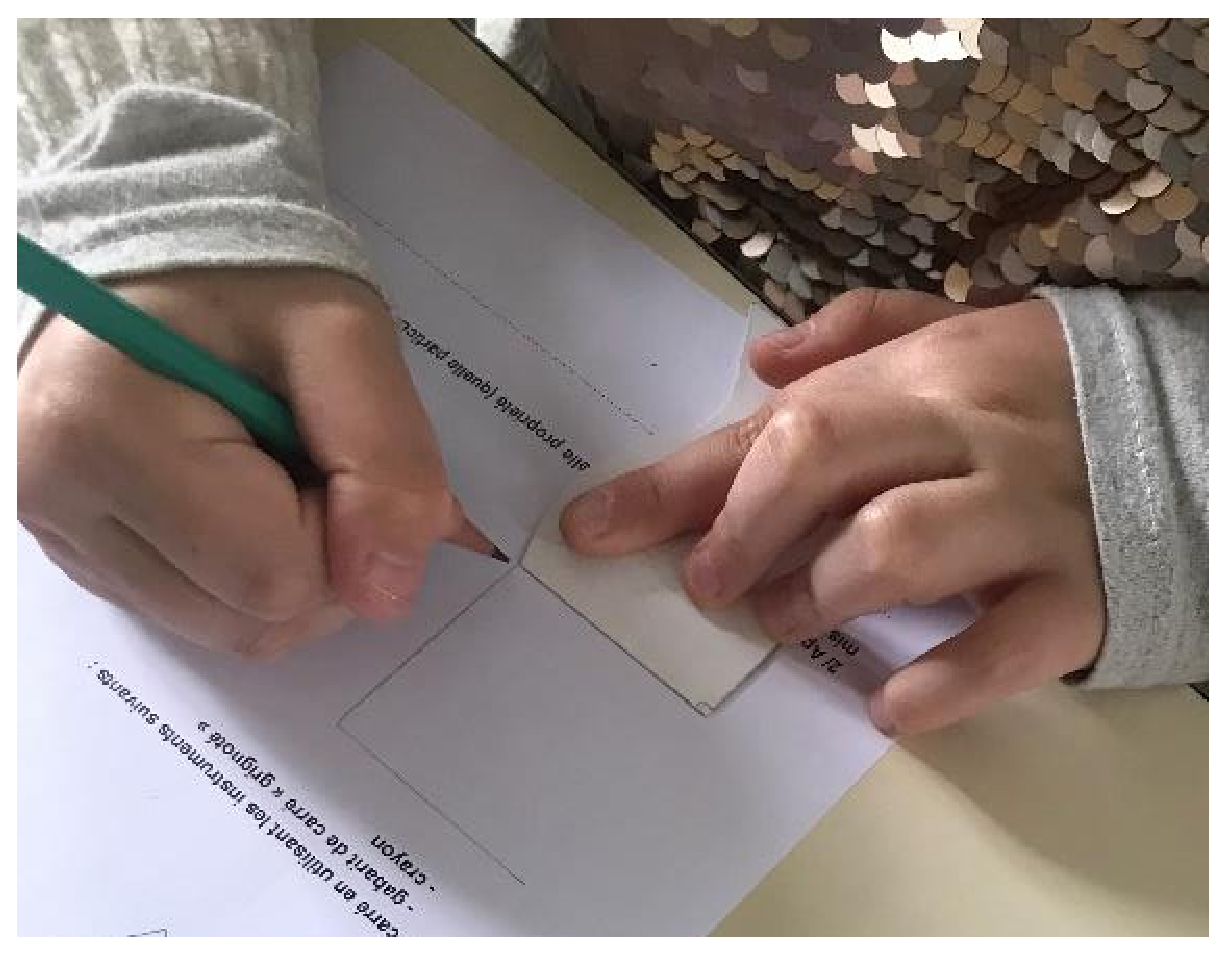
\includegraphics[height=4cm]{Geometrie_did/Images/Geo5_crpe_gabarit_E1}
   &
   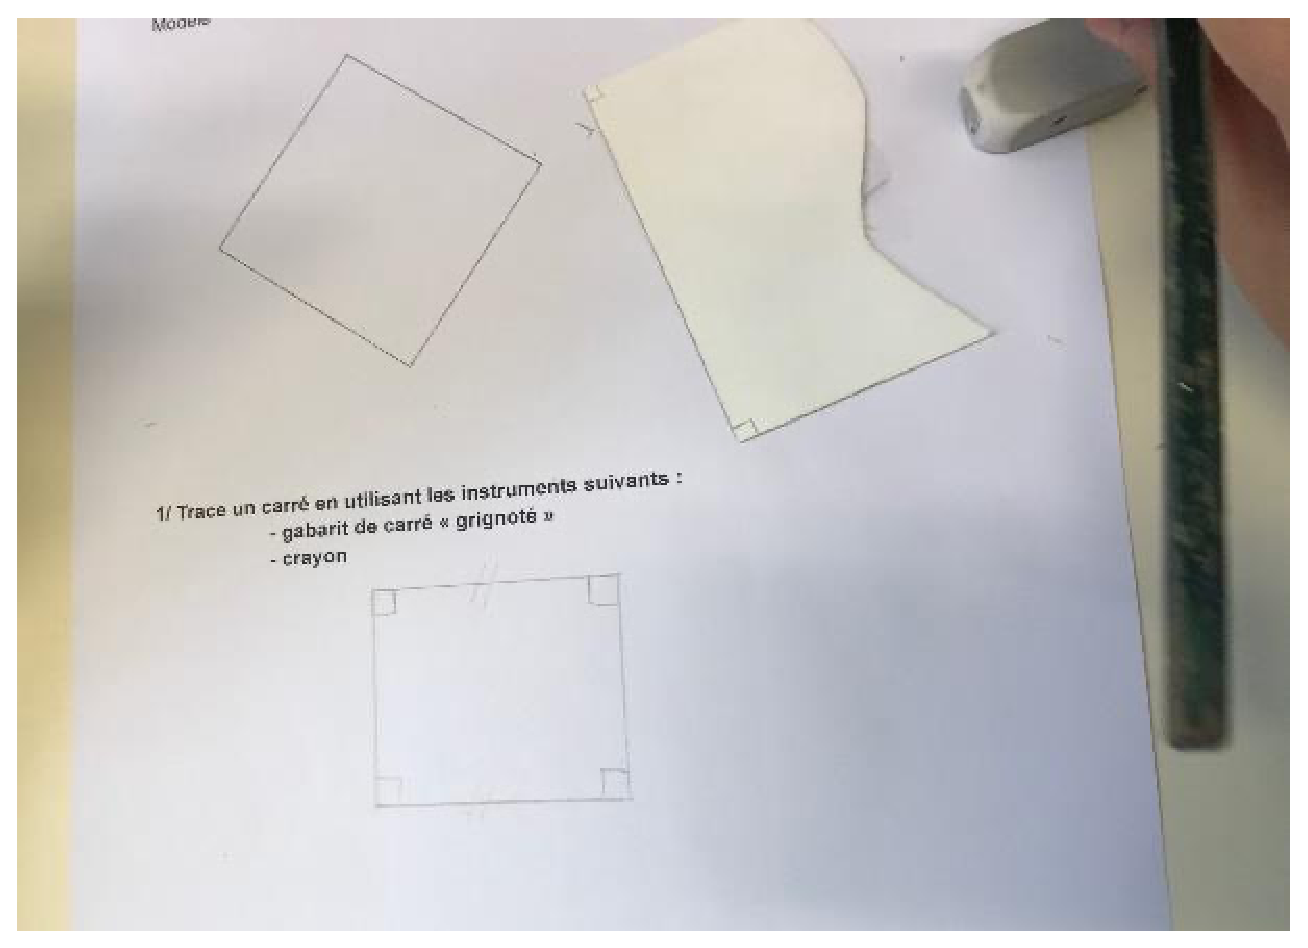
\includegraphics[height=4cm]{Geometrie_did/Images/Geo5_crpe_gabarit_E2} \\
   Élève 3. Bonne utilisation du gabarit (1)
   &
   Élève 3. Bonne utilisation du gabarit (2) \\
   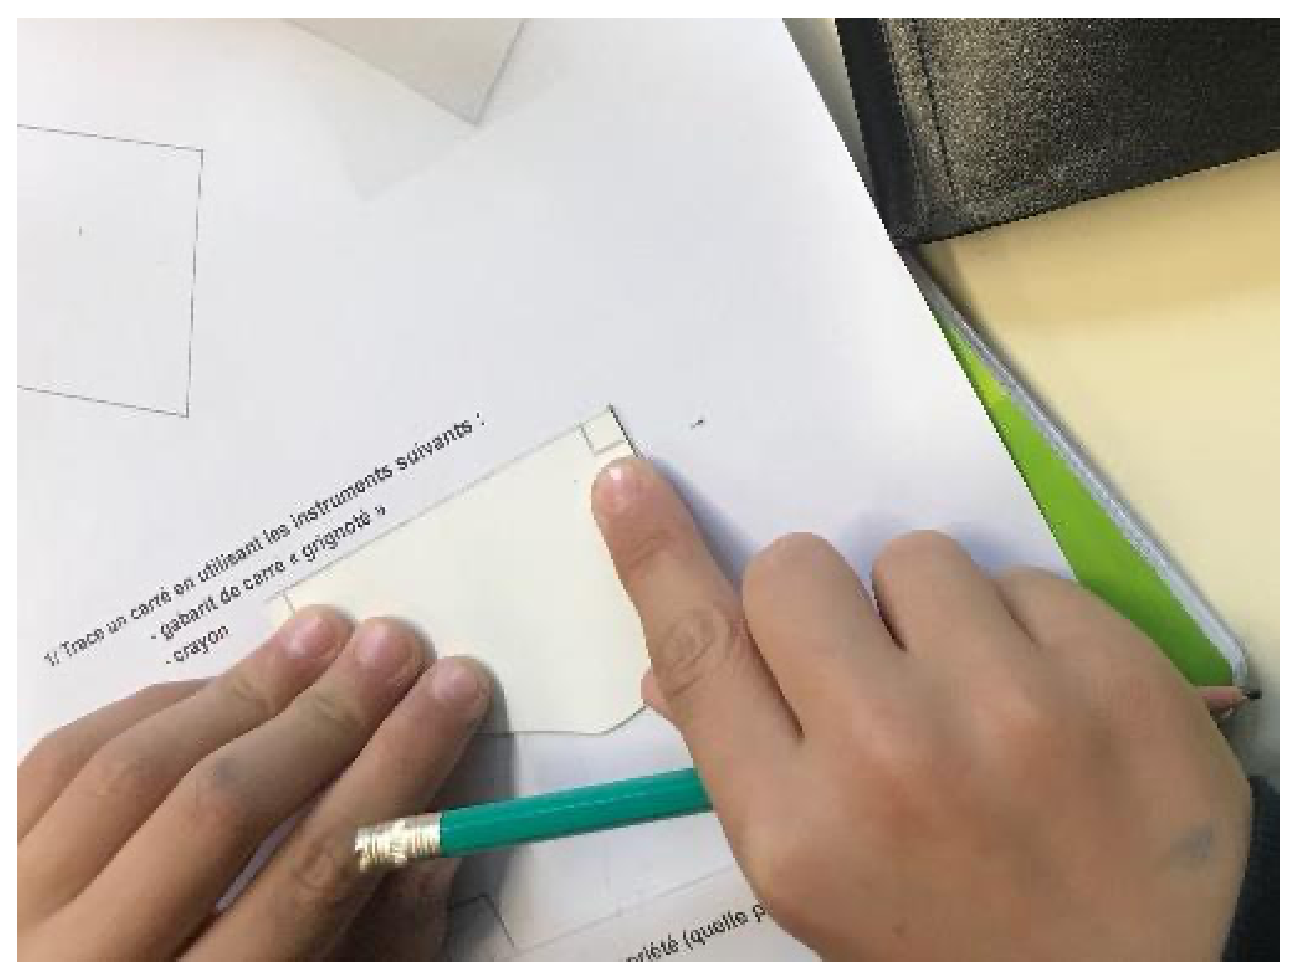
\includegraphics[height=4.2cm]{Geometrie_did/Images/Geo5_crpe_gabarit_E3}
   &
   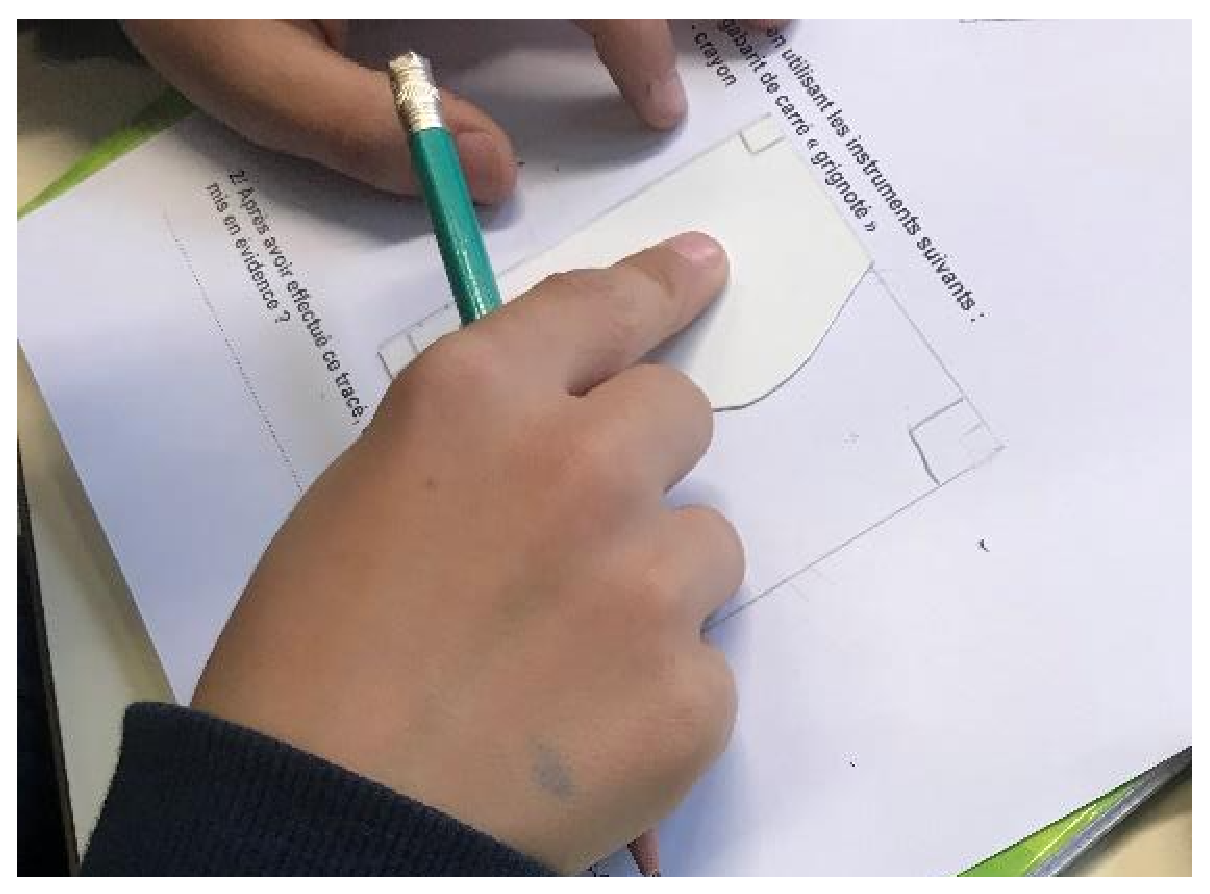
\includegraphics[height=4.2cm]{Geometrie_did/Images/Geo5_crpe_gabarit_E4} \\
\end{tabular}

{\it Gabarit grignoté 2} \\
\begin{tabular}{C{8}C{8}}
   Élève 4. Stratégie 1 : un angle à la fois
   &
   Élève 5. Stratégie 2 : deux angles à la fois \\
   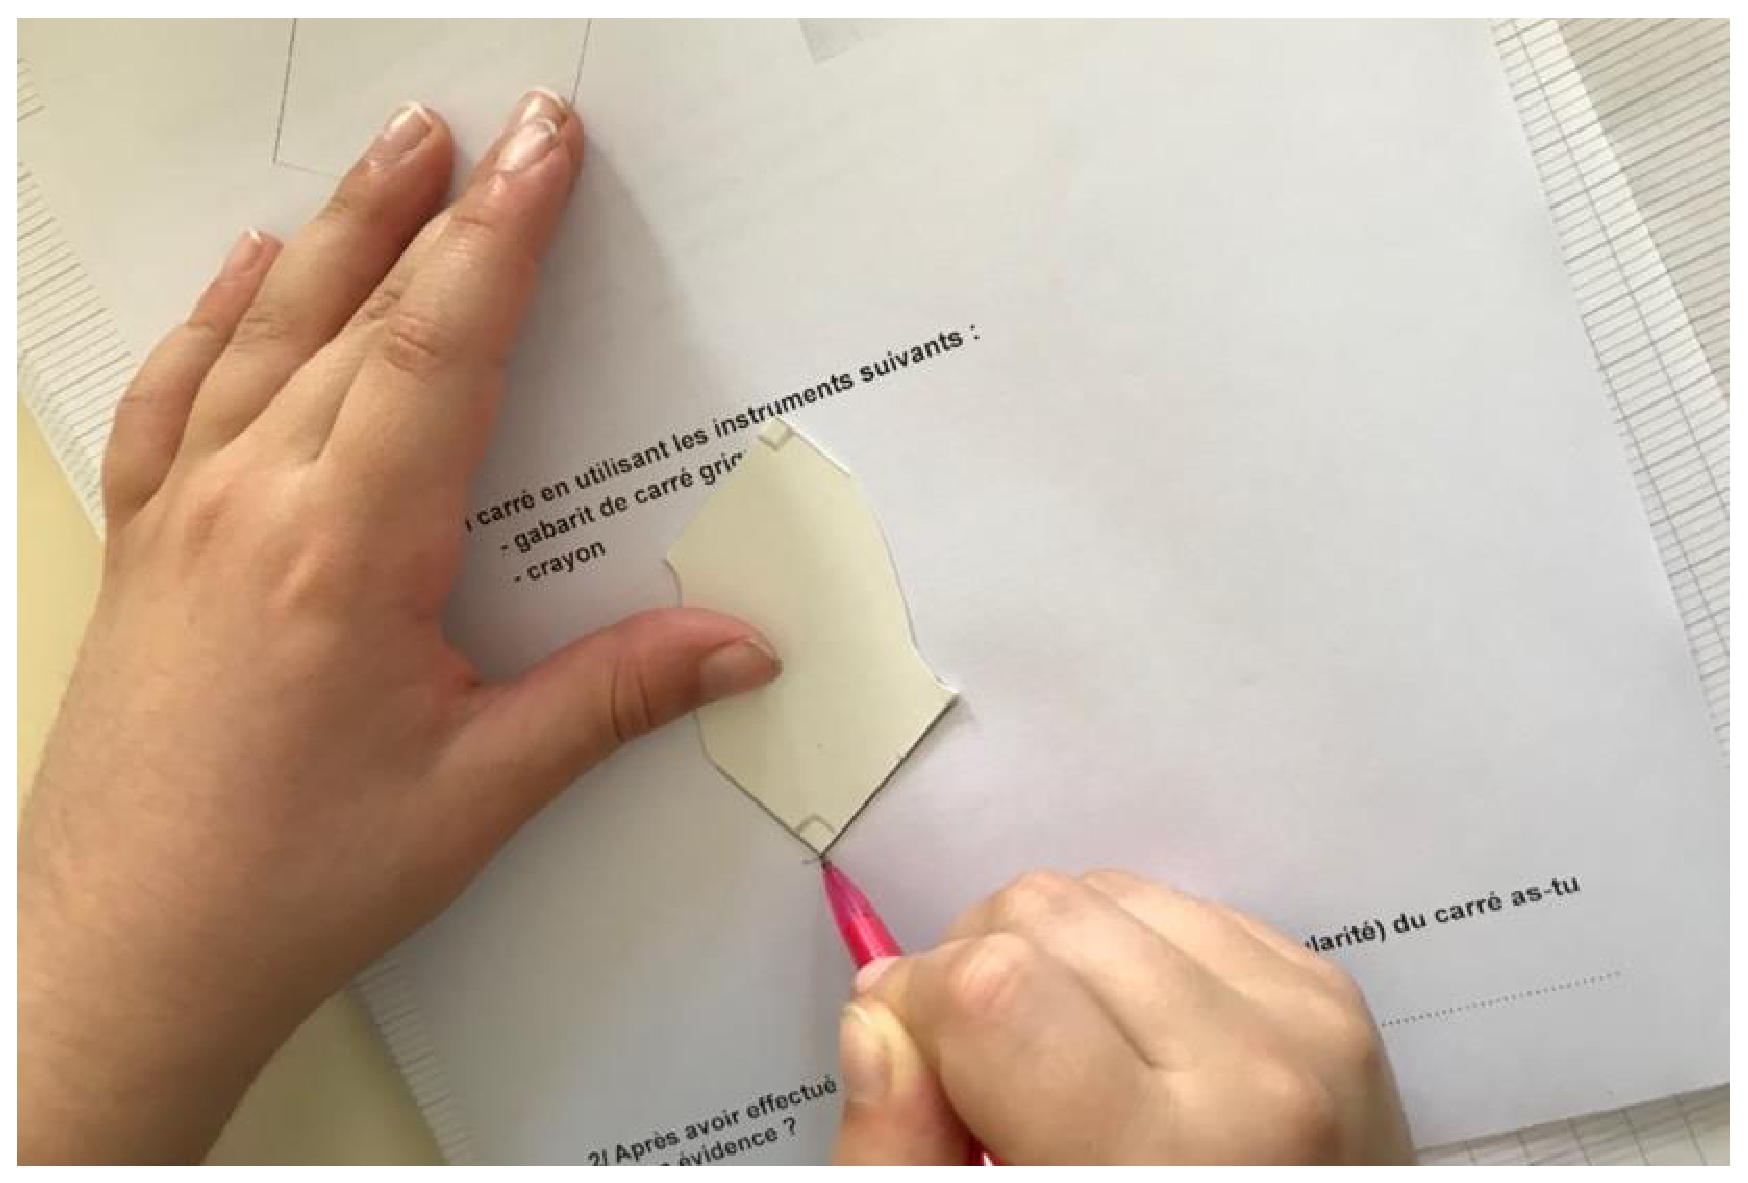
\includegraphics[height=4cm]{Geometrie_did/Images/Geo5_crpe_gabarit_E5}
   &
   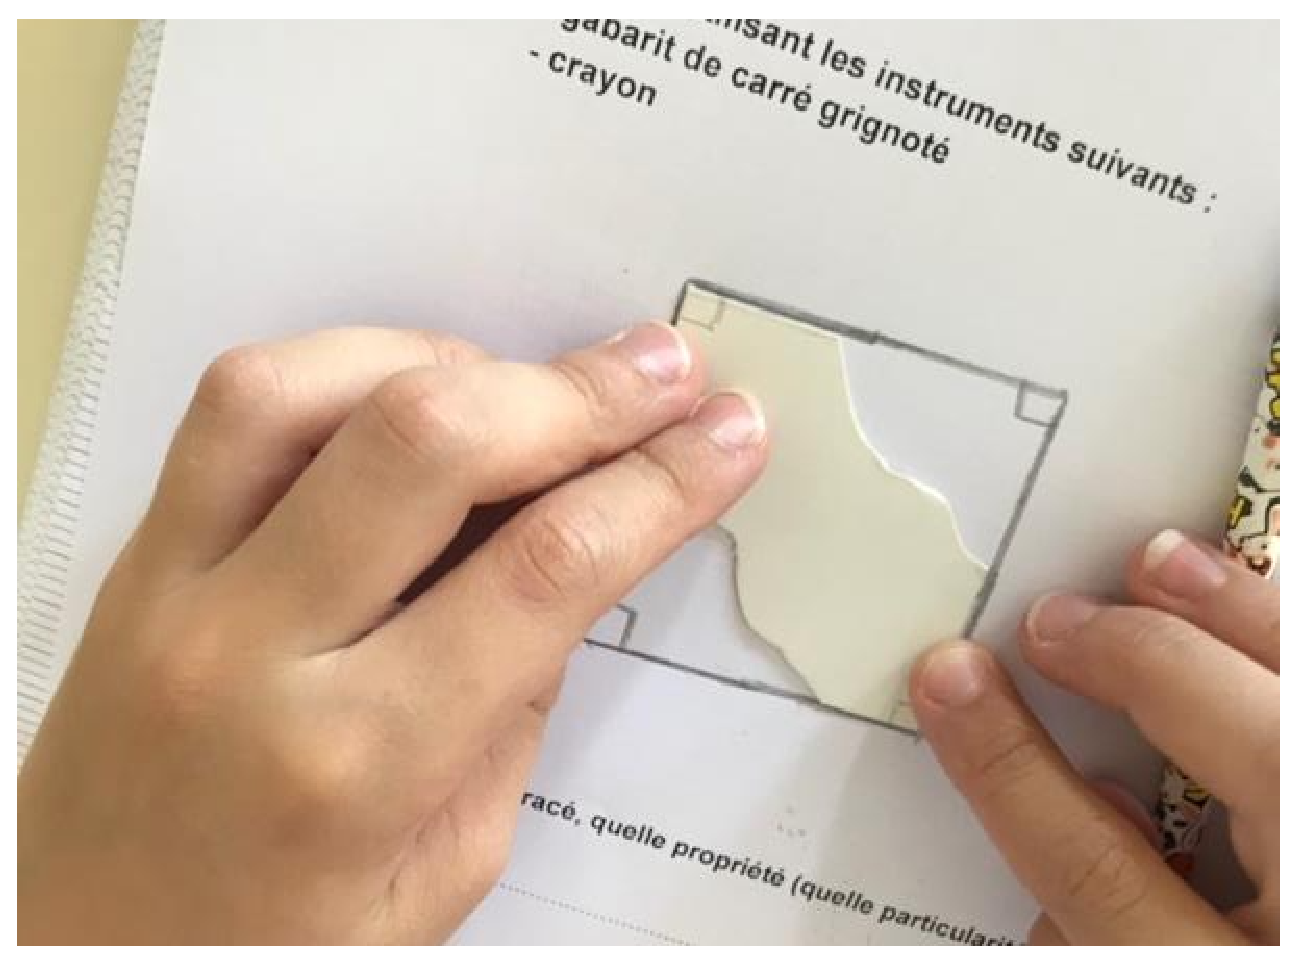
\includegraphics[height=4cm]{Geometrie_did/Images/Geo5_crpe_gabarit_E6} \\
\end{tabular}


%%%%%%%%%%%%%%%%
%%%%%%%%%%%%%%%%
\analyses

%%%%%%%%%%%%%%%%%%%%%%%%%%%%%
\begin{exercice}[Étude de productions d'élèves, Hatier concours]
   Pour chacune des erreurs ci-dessous, essayez de faire des hypothèses sur les procédures mises en place par l'élève pour les produire. Quelles sont les origines possibles de ces procédures ?
   {\setlength{\columnseprule}{0.75pt}
   \begin{multicols}{2}
   \begin{description}
      \item[Erreur 1] : préciser pour chacun des cas si les droites sont perpendiculaires. \\
      \psset{unit=0.8}
      \begin{pspicture}(3,-0.8)(5,3.5)
         \psline(3,0)(3,3)
         \psline(2,1)(4,3)
         \psline(6,0)(6,3)
         \psline(5,1)(7,1)
         \psline(8,0)(11,3)
         \psline(8,2)(10,0)
         \rput(3,-0.5){\textcolor{A1}{Oui}}
         \rput(6,-0.5){\textcolor{A1}{Oui}}
         \rput(9,-0.5){\textcolor{A1}{Non}}
      \end{pspicture} \\
      \psline(-1.2,0)(9.2,0)
      \item[Erreur 2] : tracer la perpendiculaire à la droite (d) qui passe par A. \\
       \begin{pspicture}(3,0.2)(8,3.5)
         \psline[linecolor=A1](7,0)(7,3)
         \psline(6,1)(8,2)
         \rput(7.25,2.5){$\times$ A}
         \rput(5.5,1){(d)}
      \end{pspicture} \\
      \psline(-1.2,0)(9.2,0)
      \item[Erreur 3] : tracer la perpendiculaire à la droite (d) qui passe par A. \\
       \begin{pspicture}(3,1.8)(8,3.8)
         \psline(4,3)(6.5,2)
         \rput(8,3){$\times$ A}
         \rput(5,2){$(d)$}
      \end{pspicture} \\
      \textcolor{A1}{Réponse : ce n'est pas possible} \\
      \psline(-1.4,-0.08)(9.2,-0.08)
      \item[Erreur 4] : voici un segment [AB], placer le point M milieu de ce segment. \\
      \begin{pspicture}(0,0)(7,2.8)
         \psline{|-|}(2,0)(6,2)
         \rput[r](1.8,0){A}
         \rput[l](6.2,2){B}
         \rput(4.3,0.8){\textcolor{A1}{M}}
      \end{pspicture} \\
      \psline(-1.4,0)(9.4,0)
      \item[Erreur 5] : tracer le rectangle ABCD. Tracer ensuite le segment [AC]. \\
      \begin{pspicture}(0,-1.3)(7,3)
         \pstGeonode[CurveType=polygon,PointSymbol=none,PosAngle={-135,-45,45,135},linecolor=A1](3,0){A}(6,0){B}(6,2){C}(3,2){D}
         \psline[linecolor=A1]{|-|}(3,-1)(5,-1)
         \rput[r](2.8,-1){\textcolor{A1}{$A$}}
         \rput[l](5.2,-1){\textcolor{A1}{$C$}}
      \end{pspicture} \\
      \psline(-1.4,0)(9.4,0)
      \item[Erreur 6] : reproduire la figure ci-dessous. \\
      \begin{pspicture}(3,0.5)(10,3.8)
         \pscircle(5,2){1.43}
         \psframe(4,1)(6,3)
         \pscircle[linecolor=A1](9.9,2){1.45}
         \psframe[linecolor=A1](9,1)(11,3)
         \psline[linewidth=1mm]{->}(7,2)(8,2)
         \psdots[linewidth=0.05mm,linecolor=A1](9.9,2)(9.9,2.1)(10,1.9)(10,2)(10.1,2.15) 
      \end{pspicture} \\
      \psline(-1.4,-0.08)(9.4,-0.08)
      \end{description} 
   \end{multicols}}
   {\bf Erreur 7} : écrire un texte pour permettre à quelqu'un qui ne voit pas la figure de la tracer en respectant les dimensions indiquées. \\
    \begin{minipage}{6cm}
    \begin{pspicture}(2,-0.5)(7,4.5)
         \pstGeonode[CurveType=polygon,PointSymbol=none,PointName=none](3,0){A}(5,0){B}(5,2){C}(3,2){D}
      \pstRightAngle[RightAngleSize=0.2]{A}{B}{C}
      \pstRightAngle[RightAngleSize=0.2]{B}{C}{D}
      \pstRightAngle[RightAngleSize=0.2]{C}{D}{A}
      \pstRightAngle[RightAngleSize=0.2]{D}{A}{B}
      \pscircle(5,2){2}
      \rput(4,-0.3){\scriptsize 4 cm}
      \rput(4,2.3){\scriptsize 4 cm}
      \rput(2.5,1){\scriptsize 4 cm}
      \rput(5.5,1){\scriptsize 4 cm}
   \end{pspicture}
   \end{minipage}
   \qquad
   \begin{minipage}{10cm}
      \textcolor{A1}{Patrice :} prends un compas la moitié 8 cm pour la hauteur et la largeur puis prends ta règle, au 4 cm de la hauteur et largeur trace vers le bas un trait de 4 cm puis vers la gauche de 4 cm puis la hauteur 4 cm la largeur est de 4 cm vers la droite. \\ [3mm]
      \textcolor{A1}{Géraldine :} trace un carré de 4 cm de côté, trace un cercle de 4 cm de rayon. \\ [3mm]
      \textcolor{A1}{Guillaume :} tracer un carré de 4 cm de côté ensuite tracer un cercle qui a pour centre un angle droit qui se situe en haut à droite.
   \end{minipage}
\end{exercice}


\begin{corrige}
\begin{itemize}
   \item {\bf Erreur 1 :} l'élève semble avoir compris que deux droites sont perpendiculaires si l'une des deux droites est verticale. \\
   L'horizontale et la verticale sont deux directions naturellement privilégiées dans la vie courante. D'autre part, pour beaucoup d'enfants, la perpendicularité est associée à la notion d'angle droit, droit étant lui même associé à vertical (\og tiens toi droit ! \fg).
   \item {\bf Erreur 2 :} on peut repérer la même erreur que précédemment, l'enfant a aussi pu mal utiliser son équerre. \\
   Dans ce dernier cas, il n'a peut-être pas compris l'utilisation de cet instrument : quel \og bord \fg{} je mets en correspondance avec mon dessin ? Quel \og bord \fg{} me permet de tracer la droite demandée ?
   \item {\bf Erreur 3 :} l'élève a sûrement bien placé son équerre et l'a probablement déplacée jusqu'au \og bout \fg{} de la droite. N'atteignant pas le point, il a estimé qu'il était impossible de tracer la droite. \\
   Cette démarche est directement liée à la conception que l'élève a de la représentation graphique d'une droite, il ne la perçoit pas comme étant \og infinie \fg.
   \item {\bf Erreur 4 :} la lettre représentant le point M semble à peu près correctement placée. En revanche, l'élève assimile le point à la lettre qui le nomme et n'indique pas le code qui le représente. \\
   Il peut aussi y avoir confusion du terme \og milieu \fg{} qui, dans le langage courant, signifie être entre les limites d'un objet.
   \item {\bf Erreur 5 :} l'élève a tracé {\it un} rectangle ABCD, puis {\it un} segment [AC], sans penser qu'il pourrait y avoir une relation entre les deux. \\
   Il a effectué les instructions une par une au lieu de les prendre dans leur globalité.
   \item {\bf Erreur 6 :} l'élève semble avoir construit un carré, puis, en tâtonnant (traces de la pointe du compas), a essayé de placer au mieux le cercle passant par les sommets du carré. \\
   La non-reconnaissance du lien entre les figures de base est peut-être due au fait que ce lien est à construire (les diagonales du carré).
   \item {\bf Erreur 7 :} \\
      {\bf Patrice} a identifié le cercle et un quadrilatère, commence par faire tracer le cercle puis le carré mais ses instructions ne sont pas très claires : pour le cercle, il parle simplement de compas et de la moitié de 8 cm sans préciser qu'il faut le tracer. Le carré est tracé côté par côté en donnant sa longueur et son orientation. Cet élève utilise beaucoup le langage spatial et un vocabulaire d'action en faisant référence aux instruments. Quand il utilise un vocabulaire mathématique, il y a des imprécisions et des faux sens (largeur et hauteur du cercle). \\
      {\bf Géraldine} a également identifié le carré et le cercle qu'elle caractérise convenablement, mais ne met pas en évidence les relations entre ces deux figures. L'absence de référence de relations entre le carré et le cercle a plusieurs significations : les relations ne sont pas visibles ; elle ne pense pas cela utile de le préciser, ou encore elle pense que le plus important est de décrire les figures qu'elle voit. \\
      {\bf Guillaume} a identifié le carré (par la longueur de son côté) et le cercle (par son centre), ainsi que la relation entre eux. Par conte, il ne donne pas le rayon du cercle et confond \og angle \fg{} et \og sommet de l'angle \fg{}. L'oubli du rayon est peut-être dû à une difficulté de se décentrer, et l'imprécision du vocabulaire fait penser à une trop grande influence du langage courant (angle d'une table).
\end{itemize}
\end{corrige}

\pagebreak


%%%%%%%%%%%%%%%%%%%%%%%%%%%%%%
\begin{exercice}[CRPE 2001 Limoges]
Dans une classe de cycle 3 (CM2), le maître donne l'énoncé suivant : \\
\begin{center}
\begin{minipage}{5cm}
   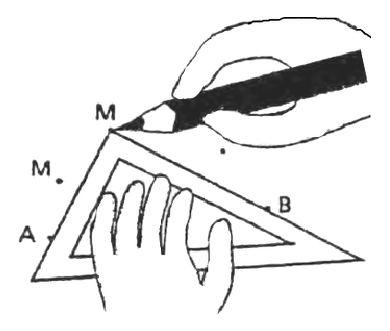
\includegraphics[width=4cm]{Geometrie_did/Images/Geo5_analyse_cercle_enonce}
\end{minipage}
\begin{minipage}{10cm}
   Observe le dessin. Louis a placé deux points A et B sur une feuille. Avec son équerre, il cherche des points M tels que la droite (AM) et la droite (BM) soient perpendiculaires. \\
   À ton tour, place deux points A et B sur une feuille blanche, et cherche au moins dix points M en faisant comme Louis. \\
   Que remarques-tu sur la position de ces points ? \\
   {\bf Optimath CM2} - Hachette Education.
\end{minipage}
\end{center}
Au bout de 15 minutes, il récupère les travaux d'élèves. Voici  six de ces travaux numérotés de (1) à (6). \\

\begin{tabular}{|p{5.5cm}|p{5.5cm}|p{5.5cm}|}
   \hline
   (1)
   &
   (2) {\small\it Je remarque que les points M forme un cercle et con peu en tracé une infinité de points}
   &
   (3) {\small\it Je remarque qu'il forme un rond} \\
   
\includegraphics[width=5cm]{Geometrie_did/Images/Geo5_analyse_cercle_T1}
   &
   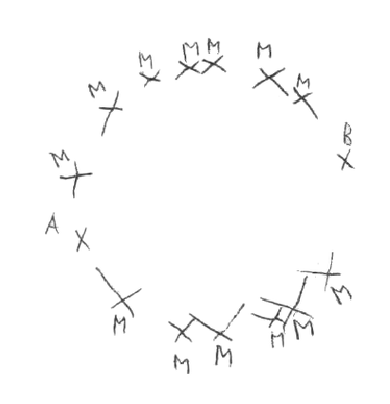
\includegraphics[width=5cm]{Geometrie_did/Images/Geo5_analyse_cercle_T2} 
   & 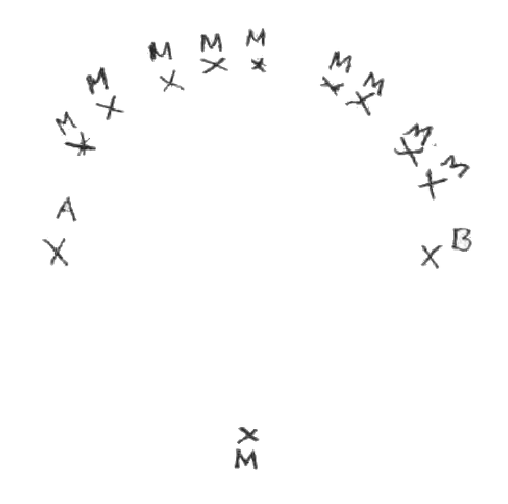
\includegraphics[width=5cm]{Geometrie_did/Images/Geo5_analyse_cercle_T3} \\
   \hline
   (4) {\small\it Les points M forme un cercle de centre identique du centre du segment AB}
   &
   (5) {\small\it Tous les points sont alignés}
   &
   (6) \\
   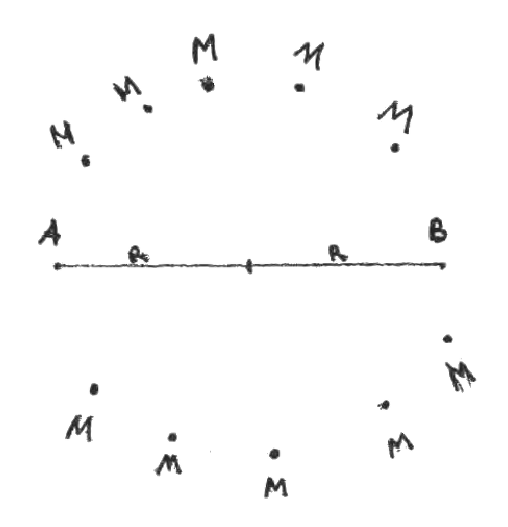
\includegraphics[width=5cm]{Geometrie_did/Images/Geo5_analyse_cercle_T4}   
   &
   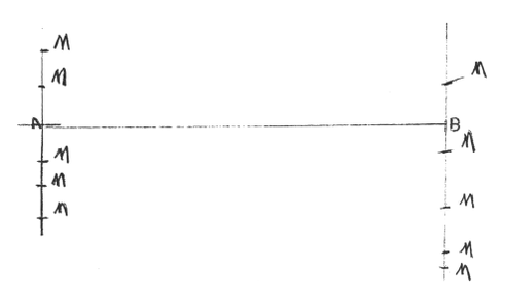
\includegraphics[width=5.5cm]{Geometrie_did/Images/Geo5_analyse_cercle_T5}
   &
   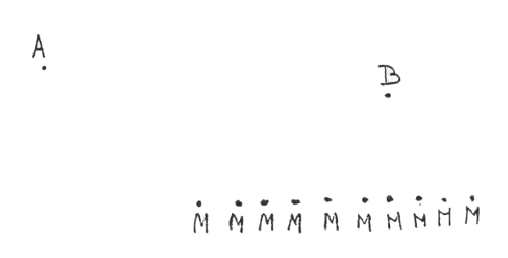
\includegraphics[width=5.5cm]{Geometrie_did/Images/Geo5_analyse_cercle_T6} \\
   \hline
\end{tabular}

\begin{enumerate}
   \item
   \begin{enumerate}
      \item Faire l'exercice proposé aux élèves sur une feuille blanche.
      \item Quelle propriété géométrique l'exercice permet-il de mettre en évidence ?
   \end{enumerate}
   \item Parmi les constructions des élèves, indiquer celles qui sont incorrectes et émettre des hypothèses sur l'origine des erreurs commises.
   \item Quelle incidence, la formulation et/ou le dessin fourni dans l'énoncé peuvent-ils avoir eue dans les productions (3) et (6) ?
\end{enumerate}
\end{exercice}

\begin{corrige}
\ \\ [-5mm]
\begin{enumerate}
   \item On effectue plusieurs tracés pour obtenir la figure suivantes : \\
   {\psset{linewidth=0.5pt}
   \begin{pspicture}(-1,-0.5)(12,4.76) 
      \pscircle[linestyle=dashed,linecolor=B2](2,2){2}
      \pspolygon(0,2)(0.17,2.81)(4,2)(0.85,3.63)
      \pspolygon(0,2)(1.98,4)(4,2)(3.14,3.64)
      \pspolygon(0,2)(3.76,2.96)(4,2)(3.96,2.42)
      \pspolygon(0,2)(0.18,1.17)(4,2)(1.3,0.13)
      \pspolygon(0,2)(2.69,0.12)(4,2)(3.67,0.9)
      \psdots[dotstyle=x,dotsize=2mm](0.17,2.81)(0.85,3.63)(1.98,4)(3.14,3.64)(3.76,2.96)(3.96,2.42)(0.18,1.17)(1.3,0.13)(2.69,0.12)(3.67,0.9)
      \psdots(0,2)(4,2)
      \rput[bl](-0.5,2){A}
      \rput[bl](4.2,2){B}
      \rput(-0.9,4){\textcolor{G1}{a)}}
      \rput(10,2.5){\begin{minipage}{9cm} \textcolor{G1}{b)} Soient A et B deux points du plan et M un troisième point du plan tel que l'angle $\widehat{\text{AMB}}$ soit un angle droit, alors M appartient au cercle de diamètre [AB]. \end{minipage}}
   \end{pspicture}}
   \item Les constructions incorrectes sont les constructions (1), (5) et (6). \\
   $\bullet$ {\bf Construction (1) :} tous les points placés au-dessus de (AB) sont bien placés mais les points placés en dessous de (AB) sont placés sur un demi-cercle ayant un diamètre dont A est une extrémité mais dont l'autre extrémité est le point M situé \og juste au-dessus \fg{} de B. Il est probable qu'ayant retourné son équerre afin de placer des points dans le demi-plan inférieur, l'élève a commis l'erreur de prendre un second point fixe autre que B, assez proche cependant de celui-ci. \\
   $\bullet$ {\bf Construction (5) :} l'élève a placé ses dix points sur deux droites parallèles aux bords verticaux de la feuille, mais également perpendiculaires au segment [AB] tracé. On peut émettre plusieurs hypothèses correspondant chacune à une compréhension incorrecte de l'énoncé :
   \begin{itemize}
      \item l'élève a confondu les termes et les concepts de \og perpendiculaire \fg{} et de \og verticale \fg{}, et considéré que la consigne de l'énoncé \og la droite (AM) et la droite (BM) sont perpendiculaires \fg{} signifiait que ces droites devaient être verticales ;
      \item il a interprété la consigne \og la droite (AM) et la droite (BM) sont perpendiculaires \fg{} en la complétant de sorte que pour lui elle devienne : \og la droite (AM) et la droite (BM) sont perpendiculaires à (AB) \fg{};
      \item il a mal utilisé son équerre et l'a placée de manière à avoir l'angle droit \og en A \fg{} et \og en B \fg{}.
   \end{itemize}  
    De plus, ce que dit cet élève est en partie inexact : les dix points ne sont pas tous sur une même droite, mais chaque groupe de cinq points se trouve sur une même droite. \\
   $\bullet$ {\bf Construction (6) :} les dix points sont alignés sur une droite, apparemment horizontale. Ces points ne respectent pas la consigne. Il est possible que cet élève ait essayé de faire comme sur l'image en plaçant de la même façon son équerre et en la gardant bien fixement posée sur sa feuille, il a alors pu placer dix points le long du bord inférieur de son équerre. C'est donc peut-être une interprétation erronée de la consigne \og faire comme Louis \fg, ainsi que du modèle que donne l'image, qui est à l'origine de cette erreur. 
   \item $\bullet$ {\bf Construction (3) :} l'élève a commencé par placer 9 points au dessus de (AB), comme le suggère l'image, puis a situé le dixième et dernier point en dessous, à égale distance de A et de B. Est-ce le sentiment de manquer de place pour placer un point de plus qui l'a amené à passer de l'autre côté de (AB) ? Le fait qu'il ait bien perçu que les points étaient sur \og un rond \fg, il l'a écrit, peut faire penser qu'il lui a fallu choisir un endroit pour placer un dernier point, le dixième\dots \\
   $\bullet$ {\bf Construction (6) :} l'image du manuel montre une façon de placer son équerre. L'énoncé n'indique pas que l'équerre peut, et doit changer de position et, manifestement, cet élève l'a gardée dans cette position fixe sur sa feuille.
\end{enumerate}
\end{corrige}

\bigskip


%%%%%%%%%%%%%%%%%%%%%%%%%%%%%%%
\begin{exercice}[CRPE 2003 Lille]
Cette partie est consacrée à l'étude :
\begin{itemize}
   \item D'une situation de recherche dirigée, menée par des élèves du cycle 2 \og LES POLYMINOS \fg.
   \item Puis, d'un document donné en travail individuel à des élèves de cycle 3. Il a pour titre \og LES POLYGONES \fg.
\end{itemize}

\smallskip

{\bf Situation de recherche dirigée au cycle 2 : LES POLYMINOS}

\begin{center}
\fbox{
\begin{minipage}{14cm}
   Les élèves travaillent en groupe restreint (6 à 8 élèves). Le maître dirige l'atelier, les autres élèves de la classe sont en travail individuel. \\
\underline{Matériel :} pour chaque élève, des triangles équilatéraux isométriques, en nombre suffisant, découpés dans du carton. \\
\underline{Consignes données par le maître :} \og Recherchez des figures géométriques différentes en assemblant exactement par un côté les triangles mis à votre disposition. Effectuez la recherche avec :
   \begin{itemize}
      \item 3 triangles
      \item 4 triangles
      \item 5 triangles \fg.
   \end{itemize}
\end{minipage}}
\end{center}

\begin{enumerate}
   \item Quelles sont les solutions possibles avec 3 triangles ? avec 4 triangles ? \\
   Indiquer le nombre de solutions et les dessiner à main levée.
   \item Quels sont les éléments importants de la consigne sur lesquels l'enseignant devra insister avant de faire commencer la recherche ?
   \item Indiquer une difficulté que peuvent rencontrer les élèves ? Quelle aide pourrait alors apporter l'enseignant ?
   \item Pourquoi avoir choisi de mener cette recherche en groupe restreint et non pas en classe entière ? Justifier.
   \item Quelle trace élaborer en fin de séance ?
\end{enumerate}

\smallskip

{\bf Situation de recherche dirigée au cycle 3 : LES POLYGONES}

\begin{center}
\fbox{
\begin{minipage}{14cm}
   Les élèves travaillent en groupe restreint (6 à 8 élèves). Le maître dirige l'atelier, les autres élèves de la classe sont en travail individuel. \\
\underline{Matériel :} annexe \og LES POLYGONES \fg{} distribuée à chaque élève par le maître. \\  
\underline{Consignes données par le maître :} \og Répondez aux questions du document que je viens de distribuer. \fg \\   
\underline{Déroulement de la séance :} travail individuel, à l'issue duquel le maître effectue une correction collective. Il prolonge l'exercice en demandant : \\
   \og Parmi les figures géométriques a, b, c, d, e, f, g, h et i, quelles sont celles que vous
pouvez nommer ? \fg
\end{minipage}}
\end{center}

\begin{enumerate}
   \item Quelles sont les compétences qui doivent être acquises par les élèves pour pouvoir répondre :
   \begin{itemize}
      \item à la question I du document élève ?
      \item aux questions a), c) et d ) de la question II du document élève ?
   \end{itemize}
   \item Que cherche à vérifier l'enseignant avec la question b) du II du document élève ?
   \item A la question d) du II du document, un élève a volontairement laissé les 3 propositions, qu'en pensez-vous ?
   \item Répondre à la question posée par le maître après la correction collective (cf. encadré ci-dessus). Que permet de mettre en évidence cette question ?
\end{enumerate}

\begin{center}
\fbox{
\begin{minipage}{16cm}
   \smallskip
   \begin{center}
      {\large LES POLYGONES}
   \end{center}   
   {\bf I. Regarde les 7 pièces  numérotées du tangram.}
   \begin{center}
   {\psset{unit=0.6}
   \begin{pspicture}(0,0)(4,4)
      \psframe(0,0)(4,4)
      \psline(0,0)(4,4)
      \psline(3,1)(0,4)
      \psline(2,0)(4,2)
      \psline(2,0)(1,1)
      \psline(3,1)(3,3)
      \rput(2,3.25){1}
      \rput(0.75,2){2}
      \rput(2.6,2){3}
      \rput(3.5,2.5){4}
      \rput(2,1){5}
      \rput(1,0.4){6}
      \rput(3.3,0.5){7}
   \end{pspicture}}
   \end{center}
   Retrouve ces 7 pièces dans chaque figure en les numérotant de la même manière que dans le tangram.
   \begin{center}
   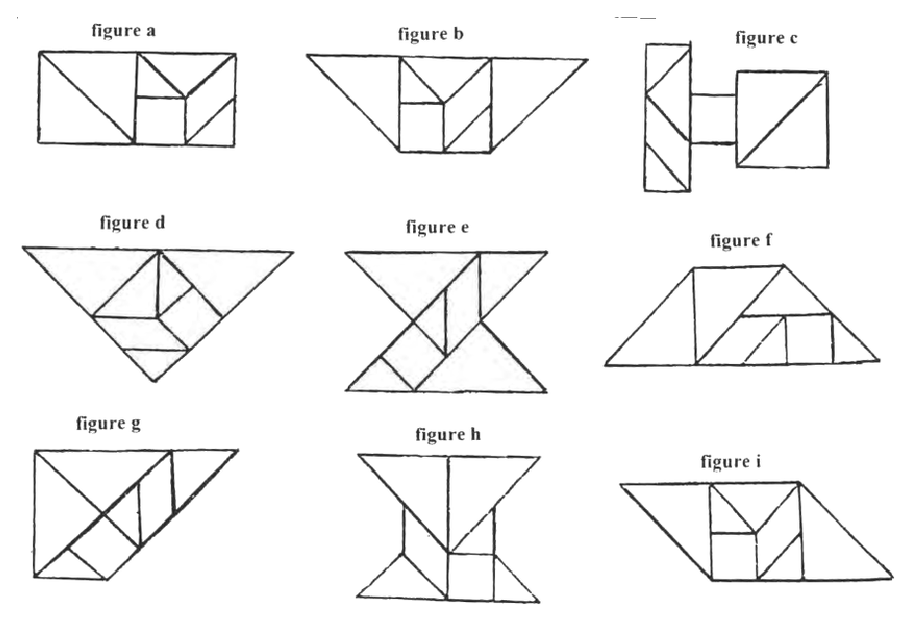
\includegraphics[width=15cm]{Geometrie_did/Images/Geo5_analyse_polygones}
\end{center}
   {\bf II. Réponds aux questions en barrant les réponses fausses.} \\
   \begin{enumerate}
      \item[a)] Que sont les polygones numérotés dans le tangram 1, 2, 3, 6 et 7 ? \\
      Des carrés \hfill Des triangles équilatéraux \hfill Des triangles rectangles isocèles
      \item[b)] En quoi sont-ils différents ? \\
      Par leur forme \hfill Par leurs dimensions
      \item[c)] Qu'est-ce que le polygone numéroté 4 dans le tangram ? \\
      Un losange \hfill Un carré \hfill Un parallélogramme
      \item[d)]  Qu'est-ce que le polygone numéroté 5 dans le tangram ? \\
      Un losange \hfill Un carré \hfill Un parallélogramme \\
   \end{enumerate}  
\end{minipage}
}
\end{center}
\end{exercice}

\begin{corrige}
{\bf Situation de recherche dirigée au cycle 2 : LES POLYMINOS} \\
\begin{enumerate}
   \item Avec trois triangle, on obtient une seule solution :
   {\psset{unit=0.8}
   \begin{pspicture}(-1,0)(4,2)
      \pspolygon(0,0)(2,0)(1,1.73)
      \pspolygon(2,0)(3,1.73)(1,1.73)
      \pspolygon(3,1.73)(2,0)(4,0)
   \end{pspicture}} \\
   Avec quatre triangles, on obtient trois solutions, que l'on construit à partir de la solution précédente à laquelle on ajoute un triangle équilatéral : \\
   {\psset{unit=0.8}
   \begin{pspicture}(0,-0.5)(6,1.5)
      \pspolygon(0,0)(2,0)(1,1.73)
      \pspolygon(2,0)(3,1.73)(1,1.73)
      \pspolygon(3,1.73)(2,0)(4,0)
      \pspolygon[linecolor=B2](4,0)(5,1.73)(3,1.73)
   \end{pspicture}
   \qquad
   \begin{pspicture}(0,-0.5)(5,3.5)
      \pspolygon(0,0)(2,0)(1,1.73)
      \pspolygon(2,0)(3,1.73)(1,1.73)
      \pspolygon(3,1.73)(2,0)(4,0)
      \pspolygon[linecolor=B2](3,1.73)(2,3.46)(1,1.73)  
   \end{pspicture}
   \qquad 
   \begin{pspicture}(0,-2.5)(4.5,1.5)
      \pspolygon(0,0)(2,0)(1,1.73)
      \pspolygon(2,0)(3,1.73)(1,1.73)
      \pspolygon(3,1.73)(2,0)(4,0)
      \pspolygon[linecolor=B2](2,0)(0,0)(1,-1.73) 
   \end{pspicture}}
   \item L'enseignant devra préciser ce qu'il appelle \og assembler les triangles exactement par un côté \fg{} en disant que deux sommets doivent également coïncider, et en présentant un exemple et des contre exemples avec des dessins. Il peut également préciser ce qu'il appelle \og des formes géométriques différentes \fg. \\
   {\psset{unit=0.8}
   \begin{pspicture}(0,0)(3,2)
      \pspolygon(0,0)(2,0)(1,1.73)
      \pspolygon(2,0)(3,1.73)(1,1.73)
   \end{pspicture}
   correct ; 
   \begin{pspicture}(-2,0)(2.5,3)
      \pspolygon(0,0)(2,0)(1,1.73)
      \pspolygon[linecolor=B2](1.34,1.14)(0.36,2.86)(2.3,2.84)
   \end{pspicture}
   et
   \begin{pspicture}(-0.5,0)(4.2,2)
      \pspolygon(0,0)(2,0)(1,1.73)
      \pspolygon[linecolor=B2](4,0)(2,0)(3,1.73)
   \end{pspicture}
   incorrects}
    \item Les élèves peuvent rencontrer des difficultés à identifier les ressemblances et les différences des assemblages qu'ils réalisent. Il serait bon de laisser du papier calque à disposition. Mais cette difficulté, naturelle en cycle 2, n'a pas à être levée individuellement ou collectivement dans la phase de recherche, elle sera prise en compte au moment de la mise en commun des différentes propositions des élèves. \\
Les élèves peuvent également avoir une certaine difficulté à organiser leur recherche, ici le maître peut apporter une aide individualisée en proposant à certains élèves de partir de l'assemblage qu'ils ont réalisé avec 3 triangles et de positionner le 4\up{ème} triangle aux différents endroits possibles.
   \item L'enseignant a choisi de mener cette recherche en groupe restreint et non en classe entière sans doute pour pouvoir apporter une aide individualisée à ses élèves et peut-être pour favoriser les échanges entre les élèves.
   \item Les élèves peuvent élaborer un document présentant les assemblages obtenus, soit en les dessinant à main levée ou sur une feuille pointée en réseau triangulaire, soit par collage. Sur ce document, il serait intéressant que les élèves écrivent une phrase liée aux objectifs que l'enseignant a défini pour cette séance.
\end{enumerate}

\medskip
{\bf Situation de recherche dirigée au cycle 3 : LES POLYGONES} \\
\begin{enumerate}
   \item \textcolor{A2}{$\bullet$} Question I : identifier une figure parmi d'autres figures.       
   \begin{itemize} 
      \item Questions a), c) et d ) de la question II : reconnaître et nommer les figures usuelles.
   \end{itemize}
   \item L'enseignant veut s'assurer que ses élèves identifient bien les propriétés spécifiques des triangles rectangles isocèles (angle droit, égalité des longueurs de 2 côtés), indépendamment de leur taille.
   \item L'élève a raison car un carré est un losange particulier, qui est aussi un parallélogramme particulier.
   \item La figure a est un rectangle, la figure d est un triangle rectangle isocèle, et la figure i est un parallélogramme. Cette question permet de mettre en évidence la capacité des élèves à envisager un assemblage de figures comme une figure unique. On pourrait également accepter que les figures b et f sont des trapèzes, même si ce n'est pas au programme.
\end{enumerate}
\end{corrige}
   
\bigskip


%%%%%%%%%%%%%%%%%%%%%%%%%%%%%%
\begin{exercice}[CRPE 2002 Dijon]
Un enseignant de cycle 3 a proposé les deux exercices donnés ci-dessous. Il a formulé la consigne suivante : \og Construisez le symétrique des figures par rapport à la droite tracée en gras \fg. II a veillé au préalable à ce que la seule ressource disponible soit la règle.
\begin{enumerate}
   \item Quelle est la compétence évaluée dans les deux exercices proposés aux élèves ?
   \item Citez deux procédures qu'un élève de cycle 3 peut utiliser pour résoudre cet exercice.
    \item Pour chaque élève (A, B, C et D), repérez les erreurs et les réussites dans les productions proposées.
    \item Quel matériel pourrait-on donner aux élèves afin qu'ils puissent vérifier s'ils ont tracé la bonne figue par symétrie ?
\end{enumerate}
\begin{center}
   \hspace*{-0.75cm}
   \psset{unit=0.35,linewidth=0.4mm}
   \begin{pspicture}(12,22)
      \rput(12,19.5){\bf Élève A}
      \psframe[fillstyle=solid,fillcolor=lightgray!50,linewidth=0](0,0)(12,8)
      \psgrid[subgriddiv=0,gridlabels=0](0,0)(12,18)
      \psline(0,8)(12,8)
      \pspolygon(4,0)(10,5)(5,3)(2,4)%
      \pspolygon(2,12)(10,11)(5,13)(4,16)
      \psdots[linewidth=0.3mm](2,12)(10,11)(5,13)(4,16)
   \end{pspicture}
   \begin{pspicture}(12,22)
      \pspolygon[fillstyle=solid,fillcolor=lightgray!50,linewidth=0](0,0)(12,0)(12,12)
      \psgrid[subgriddiv=0,gridlabels=0](0,0)(12,18)
      \psline(0,0)(12,12)
      \psline[linewidth=0.6mm](9,5)(9,8)(11,8)
      \psline[linewidth=0.6mm](9,7)(10,7)%
      \psline(9,11)(8,9)(5,12)
   \end{pspicture}
   \quad
   \begin{pspicture}(12,22)
      \rput(12,19.5){\bf Élève B}
      \psframe[fillstyle=solid,fillcolor=lightgray!50,linewidth=0](0,0)(12,8)
      \psgrid[subgriddiv=0,gridlabels=0](0,0)(12,18)
      \psline(0,8)(12,8)
      \pspolygon(4,0)(10,5)(5,3)(2,4)%
      \pspolygon(2,12)(5,13)(10,11)(4,18)
   \end{pspicture}
   \begin{pspicture}(12,22)
      \pspolygon[fillstyle=solid,fillcolor=lightgray!50,linewidth=0](0,0)(12,0)(12,12)
      \psgrid[subgriddiv=0,gridlabels=0](0,0)(12,18)
      \psline(0,0)(12,12)
      \psline[linewidth=0.6mm](9,5)(9,8)(11,8)
      \psline[linewidth=0.6mm](9,7)(10,7)%
      \psline[linewidth=0.6mm](6,9)(8,9)(8,12)
      \psline[linewidth=0.6mm](8,10)(7,10)
   \end{pspicture}
   \hspace*{-0.75cm}
   \end{center}
   \begin{center}
   \hspace*{-0.75cm}
   \psset{unit=0.35,linewidth=0.4mm}
   \begin{pspicture}(12,22)
      \rput(12,19.5){\bf Élève C}
      \psframe[fillstyle=solid,fillcolor=lightgray!50,linewidth=0](0,0)(12,8)
      \psgrid[subgriddiv=0,gridlabels=0](0,0)(12,18)
      \psline(0,8)(12,8)
      \pspolygon(4,0)(10,5)(5,3)(2,4)%
      \pspolygon(2,12)(5,13)(10,11)(4,16)
      \psdots[linewidth=0.3mm](2,12)(10,11)(5,13)(4,16)
   \end{pspicture}
   \begin{pspicture}(12,22)
      \pspolygon[fillstyle=solid,fillcolor=lightgray!50,linewidth=0](0,0)(12,0)(12,12)
      \psgrid[subgriddiv=0,gridlabels=0](0,0)(12,18)
      \psline(0,0)(12,12)
      \psline[linewidth=0.6mm](9,5)(9,8)(11,8)
      \psline[linewidth=0.6mm](9,7)(10,7)%
      \psline[linewidth=0.6mm](4,5)(4,8)(2,8)
      \psline[linewidth=0.6mm](4,7)(3,7)
      \psdots[linewidth=0.2mm](4,8)(2,8)(2,5)(3,7)
   \end{pspicture}
   \quad
   \begin{pspicture}(12,22)
      \rput(12,19.5){\bf Élève D}
      \psframe[fillstyle=solid,fillcolor=lightgray!50,linewidth=0](0,0)(12,8)
      \psgrid[subgriddiv=0,gridlabels=0](0,0)(12,18)
      \psline(0,8)(12,8)
      \pspolygon(4,0)(10,5)(5,3)(2,4)%
      \pspolygon(0.4,13.2)(4,9)(9,14.2)(5,12)
   \end{pspicture}
   \begin{pspicture}(12,22)
      \pspolygon[fillstyle=solid,fillcolor=lightgray!50,linewidth=0](0,0)(12,0)(12,12)
      \psgrid[subgriddiv=0,gridlabels=0](0,0)(12,18)
      \psline(0,0)(12,12)
      \psline[linewidth=0.6mm](9,5)(9,8)(11,8)
      \psline[linewidth=0.6mm](9,7)(10,7)%
      \psline[linewidth=0.6mm](1,5)(1,8)(3,8)
      \psline[linewidth=0.6mm](1,7)(2,7)
      \psdots[linewidth=0.07mm](1.2,5)(2.1,5)(3.2,5)(4.2,5)(5.1,5.1)(6.2,5.1)(7.2,4.8)(8.6,5.1)
   \end{pspicture}
   \hspace*{-0.75cm}
\end{center}
\end{exercice}

\begin{corrige}
\ \\ [-5mm]
\begin{enumerate}
   \item L'objectif de cette activité est : tracer, sur papier quadrillé, la figure symétrique d'une figure donnée par rapport à une droite donnée.
   \item Globalement, les procédure possibles pour un élève de cycle 3 sont :
   \begin{itemize}
      \item le pliage ;
      \item l'utilisation d'un papier calque ;
      \item l'utilisation de la règle et du compas ;
      \item l'utilisation du quadrillage : construire le symétrique de chacun des points de la figure initiale puis tracer les segments les rejoignant ;
      \item l'utilisation du quadrillage : construire le symétrique d'un point et à partir de celui-ci reconstruire la figure initiale de proche en proche.
\end{itemize}
    \item 
    \begin{itemize}
       \item {\bf Élève A} : \\
       1) l'élève a, semble-t-il, commencé par reporter les points symétriques (présence des points), cette étape est correcte. Puis il les a reliés et c'est à ce moment qu'il a commis une erreur dans la manière de les relier entre eux (ordre erroné) ; \\
       2) un seul point est bien placé et l'axe oblique est pris en compte mais la figure n'est pas correcte : il semble avoir compté le nombre de côtés de carreaux qu'il a reportés suivant des segments obliques. Il n'a pas terminé sa figure.
       \item {\bf Élève B} : \\
       1) trois points sont bien placés mais la figure n'est pas conforme (non conservation des aires). \\
       Pour placer le quatrième point, l'élève semble utiliser le bord de la feuille et non la distance à l'axe ; \\
       2) la figure est superposable mais il a tracé la figure \og en face \fg{} d'un point fictif, il s'agit d'une symétrie centrale (étudiée en 5\up{ème}).
       \item {\bf Élève C} : \\
       1) la figure est correctement construite, apparement l'élève a commencé par construire chacun des points du polygone (présence des marques), puis les a reliés ; \\
       2) la figure est bien superposable mais l'élève semble avoir construit le symétrique à partir d'un axe vertical. On peut également penser, qu'il a placé dans un premier temps les points (présence de marques), par translation, puis il a inversé la figure.
       \item {\bf Élève D} : \\
       1) la figure ressemble, mais n'est pas isométrique et aucun élément n'est juste par rapport à l'exercice demandé. Il semble que cet élève utilise une translation un peu approximative (les sommets ne sont pas tous sur des n\oe uds du quadrillage) ; \\
       2) la figure est superposable mais il a utilisé une translation et non une symétrie : il a déterminé la distance horizontale jusqu'à l'axe de symétrie en fonction des carreaux, distance qu'il a reportée pour déterminer le point de départ de la figure symétrique.
    \end{itemize}
    \item Ici, seule la règle est disponible pour l'élève, l'objectif implicite du maître est donc certainement qu'il utilise l'une des deux dernières procédures avec utilisation du quadrillage et de la règle comme instrument de tracé.
 \end{enumerate}
\end{corrige}

\pagebreak


%%%%%%%%%%%%%%%%%%%%%%%%%%%%%%
\begin{exercice}[CRPE 2004 Martinique]
Un maître se propose de mettre en place des activités de construction de figures planes. Le projet de séquence est décrit ci-dessous. Les questions suivantes visent à étudier avec précision les dessins proposés et à conduire une analyse de ce projet de séquence.
\begin{enumerate}
   \item Niveau concerné. \\
   A quel niveau de cycle peut-on proposer cette séquence ? Justifier votre réponse en trois points.
   \item Analyse des activités 1, 2 et 3. \\
   Pour chaque activité, répertorier deux compétences à mettre en oeuvre pour la réussir. Présenter les réponses sous forme de tableau.
   \item Analyse de la séquence. \\
   Quelle logique conduit l'enseignant à proposer cette suite d'activités ?
   \item Activité 3.
   \begin{enumerate}
      \item Préciser pour cette activité les rôles des 2 instruments de dessin (règle, équerre).
      \item Donner deux difficultés prévisibles pour la construction.
      \item Donner trois difficultés prévisibles pour la rédaction du programme de construction.
      \item L'enseignant veut réaliser un bilan en fin de l'activité 3, donner 3 composantes qui vous paraissent essentielles pour ce bilan. \\
   \end{enumerate}
\end{enumerate}

{\bf Projet de séquence de géométrie.}

\begin{center}
\fbox{
\begin{minipage}{16cm}
{\bf Activité 1.} \\
Quels polygones faut-il assembler pour obtenir 2 carrés ? Tu peux utiliser le crayon à papier et le tracé à main levée sur une feuille pour rechercher les solutions à partir des dessins.
\begin{center}
   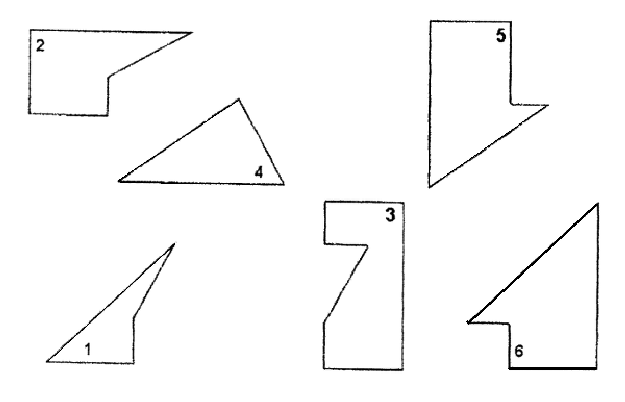
\includegraphics[width=12cm]{Geometrie_did/Images/Geo5_analyse_assemblage}
\end{center}
\end{minipage}}
\end{center}

\pagebreak
   
\begin{center}
\fbox{
\begin{minipage}{16cm}
{\bf Activité 2.} \\    
Le dessin 1 a été utilisé à partir d'un carré et des milieux de ses côtés. Reproduis le dessin 1, à l'aide de la règle non graduée, en utilisant uniquement les points du quadrillage. \\
\begin{center}
{\psset{unit=0.5}
   \begin{pspicture}(-1,-1)(7,7.5)
      \psframe(0,0)(6,6)
      \psline(0,0)(3,6)
      \psline(3,0)(6,6)
      \psline(-0.2,3)(0.3,3)
      \psline(5.8,3)(6.2,3)
      \psline(1.2,2.4)(6,0)
      \psline(2.4,4.8)(4.8,3.6)
      \rput(-0.5,6.5){A}
      \rput(-0.5,-0.5){B}
      \rput(6.5,-0.5){C}
      \rput(6.5,6.5){D}
      \rput(3,6.5){E}
      \rput(3,-0.5){F}
      \rput(3,7.5){Dessin 1}
   \end{pspicture}}
   \quad
   {\psset{unit=0.6}
   \begin{pspicture}(-3,-1)(7,6.5)
      \psgrid[subgriddiv=1,griddots=1,gridlabels=0,gridwidth=1mm](6,6)
   \end{pspicture}}
\end{center}
\end{minipage}}
\end{center}

\begin{center}
\fbox{
\begin{minipage}{16cm}
{\bf Activité 3.} \\
   1) Reproduis le dessin 1 sur cette feuille blanche à partir du nouveau dessin ABED. Instruments autorisés : règle non graduée, équerre. \\
   2) Rédige un programme de construction. \\
  \begin{center}
  {\psset{unit=0.5}
   \begin{pspicture}(-1,-1)(7,6.5)
      \psline(6,6)(0,6)(0,0)(3,6)
       \rput(-0.5,6.5){A}
      \rput(-0.5,-0.5){B}
      \rput(6.5,6.5){D}
      \rput(3,6.5){E}
   \end{pspicture}}
   \end{center}
\end{minipage}}
\end{center}
   
\begin{center}
\fbox{
\begin{minipage}{16cm}
{\bf Activité 4.} \\
   1) Reproduis le dessin 2 sur cette feuille blanche à partir du triangle ABE. Instruments autorisés : compas, règle non graduée, équerre. \\
   2) Quelles remarques peux-tu faire sur les polygones qui composent le dessin 2 ? \\
   Que remarques-tu en comparant le dessin 1 et le dessin 2 ? \\
   {\psset{unit=0.5}
   \rotatebox{26.5}{
   \begin{pspicture}(-3,-0.2)(6,6.8)
      \psline(0,0)(6,0)(6,6)(3,6)
      \psline(0,0)(3,6)
      \psline(3,0)(6,6)
      \psline(1.2,2.4)(6,0)
      \psline(2.4,4.8)(4.8,3.6)
      \psline(0,0)(6,-3)(6,0)
      \rput(6.5,0){\rotatebox{-26.5}{A}}
      \rput(-0.5,-0.5){\rotatebox{-26.5}{B}}
      \rput(6.5,-3){\rotatebox{-26.5}{E}}
      \rput(-1,6){\rotatebox{-26.5}{Dessin 2}}
   \end{pspicture}}}
   \qquad
   {\psset{unit=0.7}
   \rotatebox{26.5}{\begin{pspicture}(-2.5,-0.5)(6,3)
      \pspolygon(0,0)(6,-3)(6,0)
      \rput(6.5,0){\rotatebox{-26.5}{A}}
      \rput(-0.5,-0.5){\rotatebox{-26.5}{B}}
      \rput(6.5,-3){\rotatebox{-26.5}{E}}
   \end{pspicture}}}
\end{minipage}}
\end{center}
\end{exercice}

\begin{corrige}
\ \\ [-5mm]
\begin{enumerate}
   \item Cette séquence peut être proposée en deuxième année du cycle 3 (CM2) où on retrouve les compétences suivantes :
      \begin{itemize}
         \item utiliser les instruments pour tracer des droites parallèles et perpendiculaires ;
        \item vérifier la nature d'une figure en ayant recours aux instruments ;
         \item reproduire une figure complexe (sur papier uni, quadrillé ou pointé), à partir d'un dessin ;
         \item rédiger un programme de construction.
      \end{itemize}
   \item 
   Tableau comportant deux compétences pour chaque activité. \\ [1mm]
   \begin{CLtableau}{0.926\linewidth}{3}{c|C{5}|C{8.5}}
      \hline
      & Compétence générale  & compétence \og instrumentale \fg \\
      \hline
      1 & Reconnaître, reproduire un carré & Vérifier qu'un angle est droit en utilisant l'équerre ou un gabarit \\
      \hline
      2 & Reproduire une figure sur papier pointé, à partir d'un dessin & Utiliser la règle et l'équerre pour construire des figures planes usuelles \\
      \hline
      3 & Rédiger un programme de construction & Utiliser les instruments (règle, équerre) pour reproduire une figure sur papier uni à partir d'un modèle \\
      \hline
   \end{CLtableau}
   \item Plusieurs logiques peuvent être mises en évidence :
   \begin{itemize}
      \item utilisation progressive d'instruments dans le cadre d'une difficulté croissante. D'abord règle sur un support pointé (activité 2), puis règle et équerre sur du papier uni (activité 3), et enfin règle, équerre et compas sur du papier uni (activité 4) ;
      \item volonté de faire acquérir aux élèves des compétences spatiales dans une activité de reproduction de dessins. Reconstitution de figures à partir de pièces (activité 1), reproduction d'une figure avec l'aide d'un papier pointé (activité 2), et enfin, reproduction d'une figure sur papier uni à l'aide d'instruments de géométrie et formulation de l'action (activités 3 et 4).
    \end{itemize}
   \item 
   \begin{enumerate}
      \item La règle permet de vérifier des alignements d'objets, de tracer des segments en joignant 2 points, et de réaliser des alignements. L'équerre permet de vérifier si un angle est droit, de tracer une perpendiculaire à un segment en un point donné. On remarque qu'aucun instrument n'est dévolu à la comparaison de longueurs : est-ce pour faire réfléchir l'élève à une procédure de comparaison non numérique ? (par exemple : étalon).
      \item Il y a plusieurs \og familles \fg{} de difficultés :
      \begin{itemize}
         \item prendre l'information nécessaire pour la reproduction du dessin qui n'est pas codée explicitement : égalité de longueurs de segments, angles droits, alignements ;
         \item déterminer l'ordre des constructions à réaliser ;
         \item utiliser des instruments, en particulier l'équerre.
      \end{itemize}
      \item
      \begin{itemize}
         \item Difficulté à trouver l'ordre des différentes étapes de la construction.
         \item Difficulté à décrire une construction, en particulier dans l'élaboration de phrases souvent très complexes pour des enfants de cet âge.
         \item Difficulté à utiliser du vocabulaire géométrique efficace (perpendiculaire à un segment en un point\dots) des désignations géométriques (nommer un point, désigner un segment, une droite).
      \end{itemize}
      \item
      \begin{itemize}
         \item Reprendre collectivement la construction de la figure complexe en pointant la nécessité de bien l'analyser (ce que permet l'activité 2) et faire réaliser avec soin les différents tracés de perpendiculaires.
         \item Reprendre collectivement la rédaction du programme en introduisant le vocabulaire géométrique approprié utilisable dans de futures activités identiques.
   \end{itemize}
   \end{enumerate}
\end{enumerate}
\end{corrige}


%%%%%%%%%%%%%%%%
%%%%%%%%%%%%%%%%
\Recreation

\setcounter{exercice}{0}
\begin{exercice*}[\fbox{C1} - Explorer les formes : carré, triangle et disque]
\ \\
\begin{minipage}{10cm}
   {\it Il était un petit homme, vers les maths p.94, PS, Accès} \\ [-2mm]  
   
   {\bf Matériel :}
   \begin{itemize}
      \item une reproduction par élève du dessin du \og petit homme \fg ;
      \item les formes nécessaires pour compléter le dessin du \og petit homme \fg{} incomplet ;
      \item des formes d'un jeu de construction ;
      \item une boîte avec un trou pour passer la main. \\
   \end{itemize}
\end{minipage}
\qquad
\begin{minipage}{5cm}
   \rput(3,1){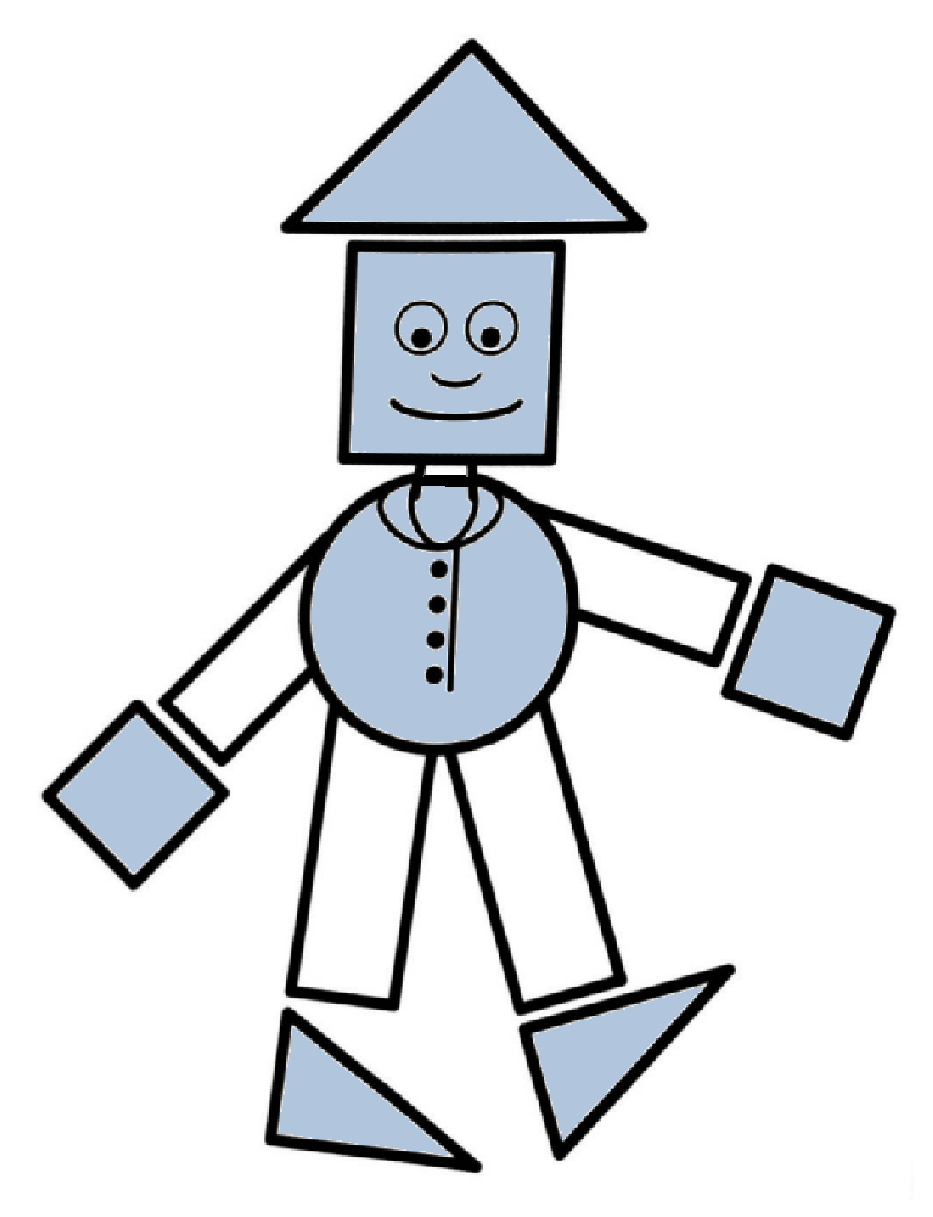
\includegraphics[width=4.5cm]{Geometrie_did/Images/Geo5_activite_bonhomme}}
\end{minipage} 

{\bf Organisation :} atelier de 4 à 6 élèves. \\ [-3mm]

{\bf Déroulement :}
\begin{enumerate}
   \item {\bf Étape 1 : nommer les formes}. \\
   Chaque élève reçoit un dessin représentant le petit homme. Les formes géométriques sont placées au centre de la table. L'enseignant chante le refrain de la chanson \og Pirouette cacahuète \fg{} dont les paroles ont été modifiées :
   
   \begin{center}
   \fbox{
   \begin{minipage}{12cm}
   \begin{multicols}{2}
      Il était un petit homme \\
      Pirouette cacahuète \\
      Il était un petit homme \\
      Qui avait un drôle de chapeau \\
      Qui avait de drôles de petites mains \\
      Qui avait de drôles de chaussures \\
      Qui avait une drôle de p'tite tête \\
      Qui avait une drôle de chemise
   \end{multicols}
   \end{minipage}
   }
   \end{center}

   Pour chaque strophe, l'enseignant présente et nomme une forme pour compléter son petit homme puis la pose sur son dessin. Il demande aux élèves de chercher une forme identique au centre de la table. \\ [-2mm]
   
\item {\bf Étape 2 : trier des formes simples}.
\begin{itemize}
   \item Trier les formes en papier utilisées pour reconstituer le petit homme. Chercher tous les disques puis tous les triangles et enfin les carrés.
   \item Compléter le classement obtenu avec des figures planes de la classe (différentes matières, tailles et couleurs). \\ [-2mm]
\end{itemize}

\item {\bf Étape 3 : reconnaître des formes géométriques par le toucher}. \\
Chaque élève dispose d'une boîte fermée dans laquelle se trouvent des figures planes. Un trou permet de passer la main pour toucher les formes à l'intérieur de la boîte. Un voile en tissu empêche de voir à l'intérieur de la boîte.
\begin{itemize}
   \item Ouvrir les boîtes et nommer les formes contenues dans sa boîte et les sortir une à une. Constater que chaque élève a les mêmes éléments : carrés, disques et triangles de différentes couleurs.
   \item Prendre tous la même forme. la manipuler en fermant les yeux et la remettre dans sa boîte.
   \item Fermer les boîtes, passer la main par le trou et explorer le contenu de la boîte. Sortir la forme de son choix, la nommer.
   \item Remettre toutes les formes dans la boîte et sortir une forme en respectant la consigne de l'enseignant. L'enseignant montre ou nomme l'objet que les élèves doivent sortir. Commencer par sortir les ronds. \\ [-2mm]
\end{itemize}
\end{enumerate}

{\bf Différentiation :} \\
Sur la table, prévoir des formes identiques à celles contenues dans la boîte. Les élèves qui ne savent pas nommer une forme peuvent la montrer. L'enseignant rappelle le nom des formes en les montrant.
\end{exercice*}


\begin{exercice*}[\fbox{C1} - Tangram]
{\it Cette séquence est téléchargeable sur \href{https://www.edumoov.com/fiche-de-preparation-sequence/34779/explorer-des-formes-des-grandeurs-des-suites-organisees/ms-gs/le-tangram}{edumoov}.}
\begin{center}
   
\includegraphics[width=15cm]{Geometrie_did/Images/Geo5_activite_edumoov1} \\
   
\includegraphics[width=15cm]{Geometrie_did/Images/Geo5_activite_edumoov2} \\ [10mm]
   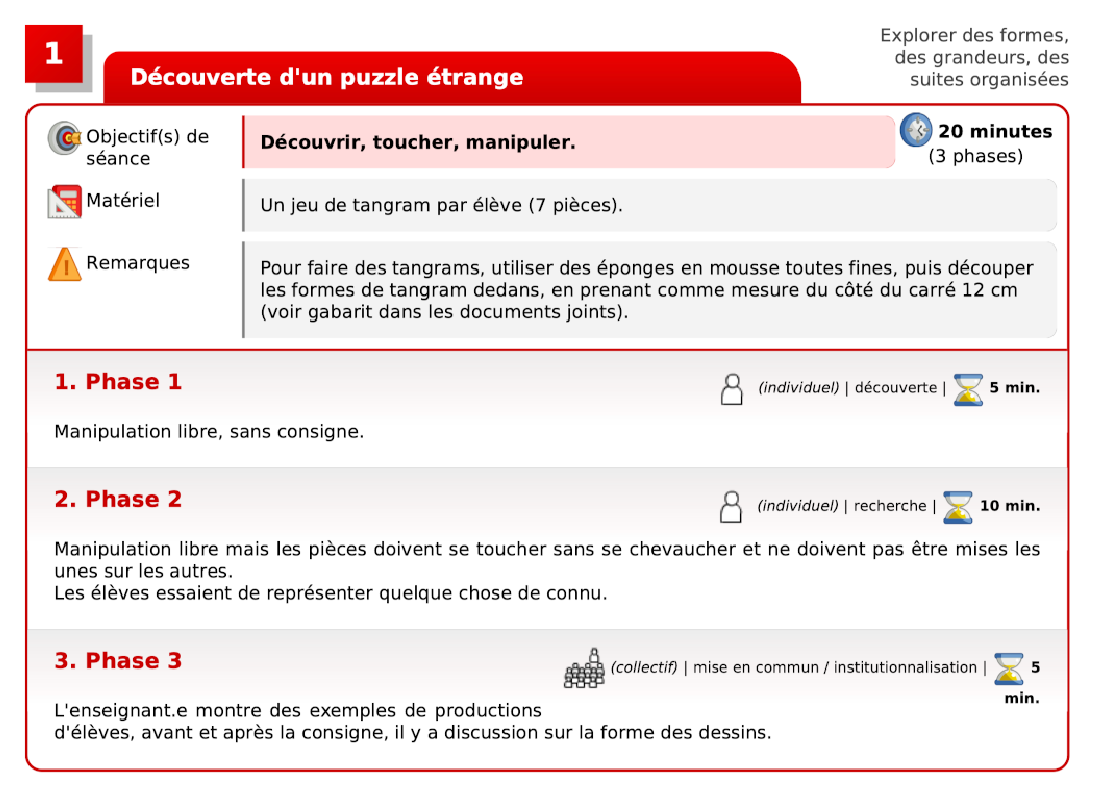
\includegraphics[width=15cm]{Geometrie_did/Images/Geo5_activite_edumoov3} \\
   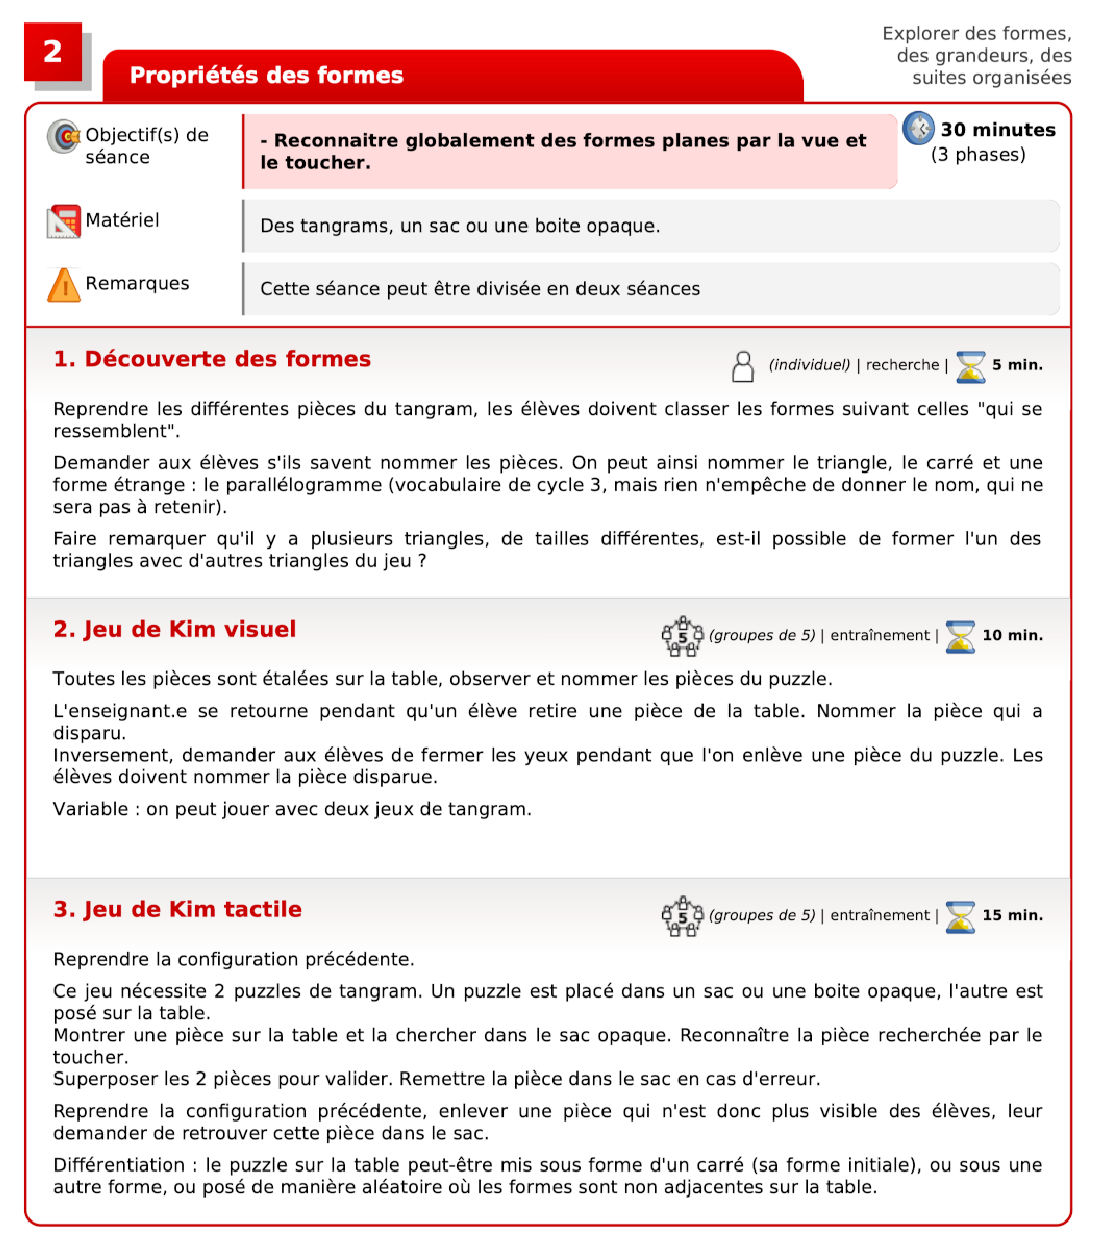
\includegraphics[width=15cm]{Geometrie_did/Images/Geo5_activite_edumoov4} \\ [10mm]
   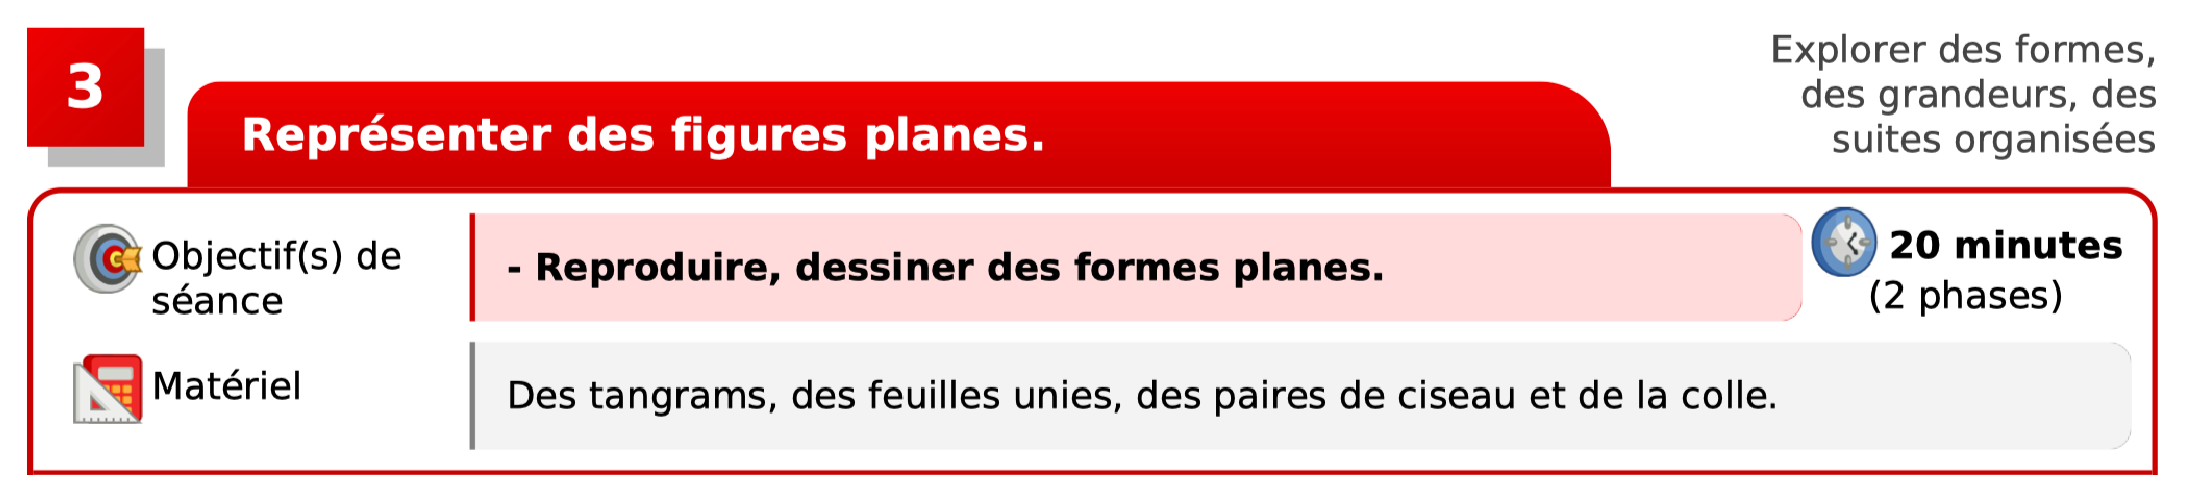
\includegraphics[width=15cm]{Geometrie_did/Images/Geo5_activite_edumoov5} \\
   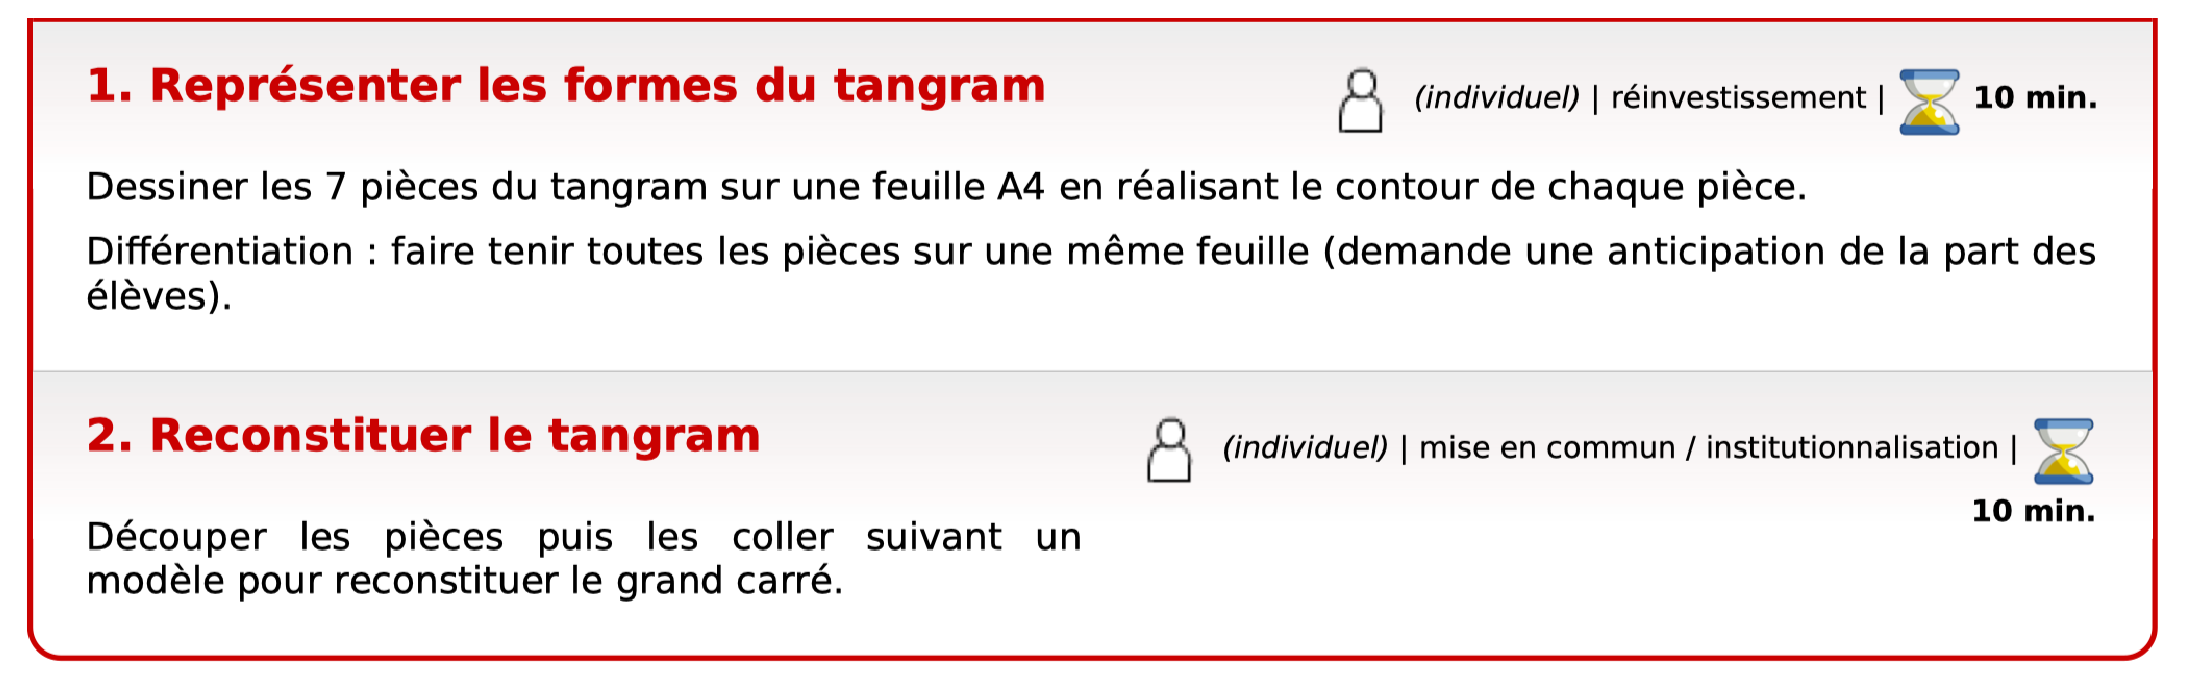
\includegraphics[width=15cm]{Geometrie_did/Images/Geo5_activite_edumoov6} \\
   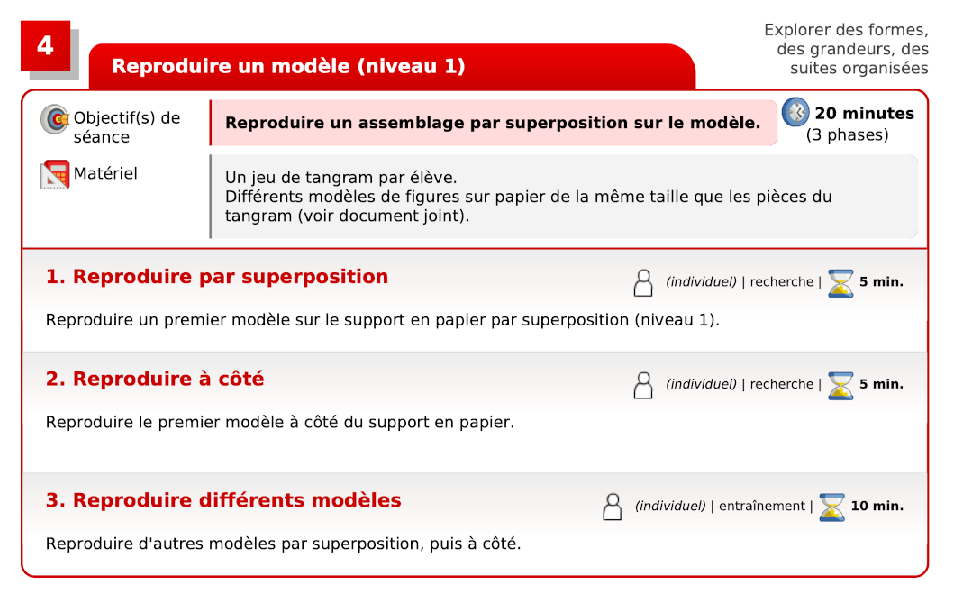
\includegraphics[width=15cm]{Geometrie_did/Images/Geo5_activite_edumoov7} \\ 
   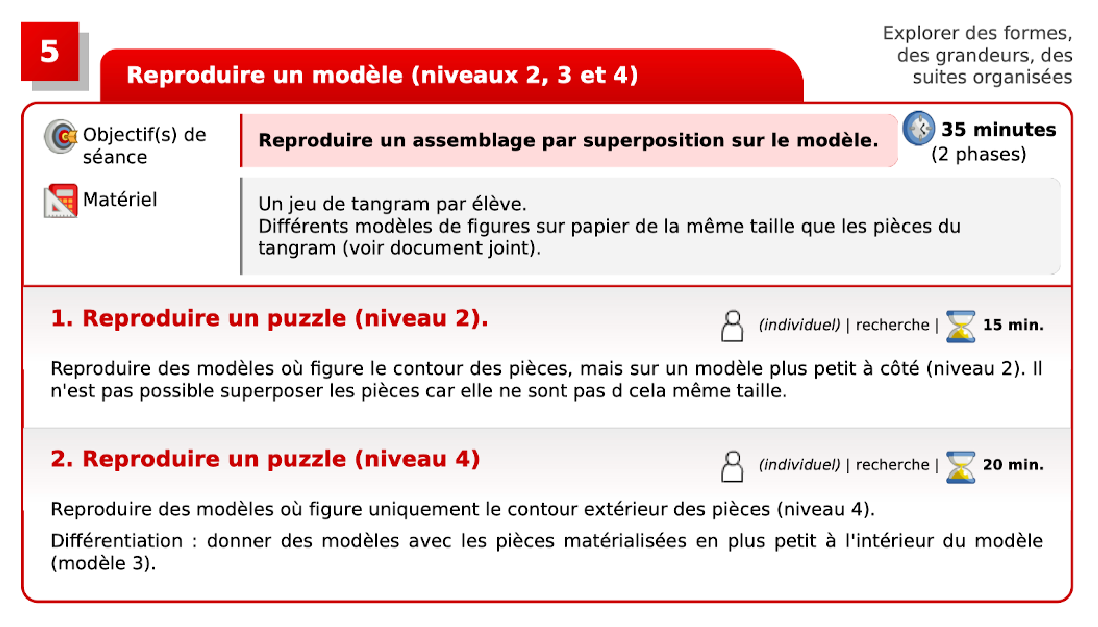
\includegraphics[width=15cm]{Geometrie_did/Images/Geo5_activite_edumoov8}
\end{center}
\end{exercice*}


\begin{exercice*}[\fbox{C2/C3} - Rallye tangram]

Pour une première approche du tangram, il est tout à fait possible de reprendre les activités proposées pour le cycle~1, à adapter en fonction de la classe, puis, lorsque les élèves ont compris le fonctionnement du tangram, on peut leur proposer un rallye mathématique qui peut prendre plusieurs formes :
\begin{itemize}
   \item un mini-rallye en une séance, par groupes, sur un nombre limité de modèles ;
   \item un rallye en fil rouge sur une période (ou plus), les élèves résolvant les modèles à leur rythme quand ils ont terminé un travail par exemple. Il remplissent une fiche individuelle.
\end{itemize}

Vous pouvez trouver des ressources à ce sujet \href{http://boutdegomme.fr/rallye-tangram-a78475195}{ici, sur le site de boutdegomme}. \\

\begin{center}
   {\textcolor{B1}{{\Large Mini rallye}}}
\end{center}

{\bf Objectif :} reconnaitre, nommer, décrire, reproduire, construire quelques figures géométriques (la construction de frises, pavages, puzzles peuvent contribuer à développer la connaissance des propriétés des figures du programme et du vocabulaire associé). Le vocabulaire et les propriétés sont sous-jacents dans l'activité. \\

{\bf Matériel et organisation :}
\begin{itemize}
   \item un tangram pour deux à trois élèves ;
   \item des modèles de tangram à réaliser ;
   \item une fiche de route pour la classe affichée au tableau.
\end{itemize}
Le jeu se fait en ilots de 4 à 5 élèves, procurer deux tangrams par ilot. \\

{\bf Historique :} ce casse-tête serait né en Chine au 16\up{è} siècle, de la maladresse d’un empereur qui, admirant un magnifique carreau de porcelaine, l’aurait laissé choir sur le sol de son palais, où il se serait brisé en sept morceaux. Voulant reconstituer l’original, il ne peut jamais y parvenir, mais il recréa à la place des milliers de figures différentes\dots \\

{\bf Règle du jeu :}
\begin{itemize}
   \item vous devez reconstituer chacune de ces formes (carré, maison, homme\dots{}), dans n'importe quel ordre grâce aux pièces du tangram. Une figure doit toujours être constituée des sept polygones et les pièces ne peuvent être que juxtaposées et non superposées ;
   \item une fois l'une des figures réalisée et vérifiée par l'enseignant(e), vous pouvez alors valider la construction dans le tableau en mettant une croix au bon endroit ! \\
\end{itemize}
   
{\bf Le tableau à remplir et les formes à reconstituer :} \\ [2mm]
{\renewcommand{\arraystretch}{1.5}
\begin{tabular}{|c|*{8}{C{1.5}|}}
  \hline
  & 1. carré &  2. maison & 3. homme & 4. voilier & 5. pull & 6. sapin & 7. usine & 8. oie \\
  \hline
  groupe 1 & & & & & & & & \\
  \hline
  groupe 2 & & & & & & & & \\
  \hline
  groupe 3 & & & & & & & & \\
  \hline
  groupe 4 & & & & & & & & \\
  \hline
  groupe 5 & & & & & & & & \\
  \hline
  groupe 6 & & & & & & & & \\
  \hline
\end{tabular}}

\pagebreak

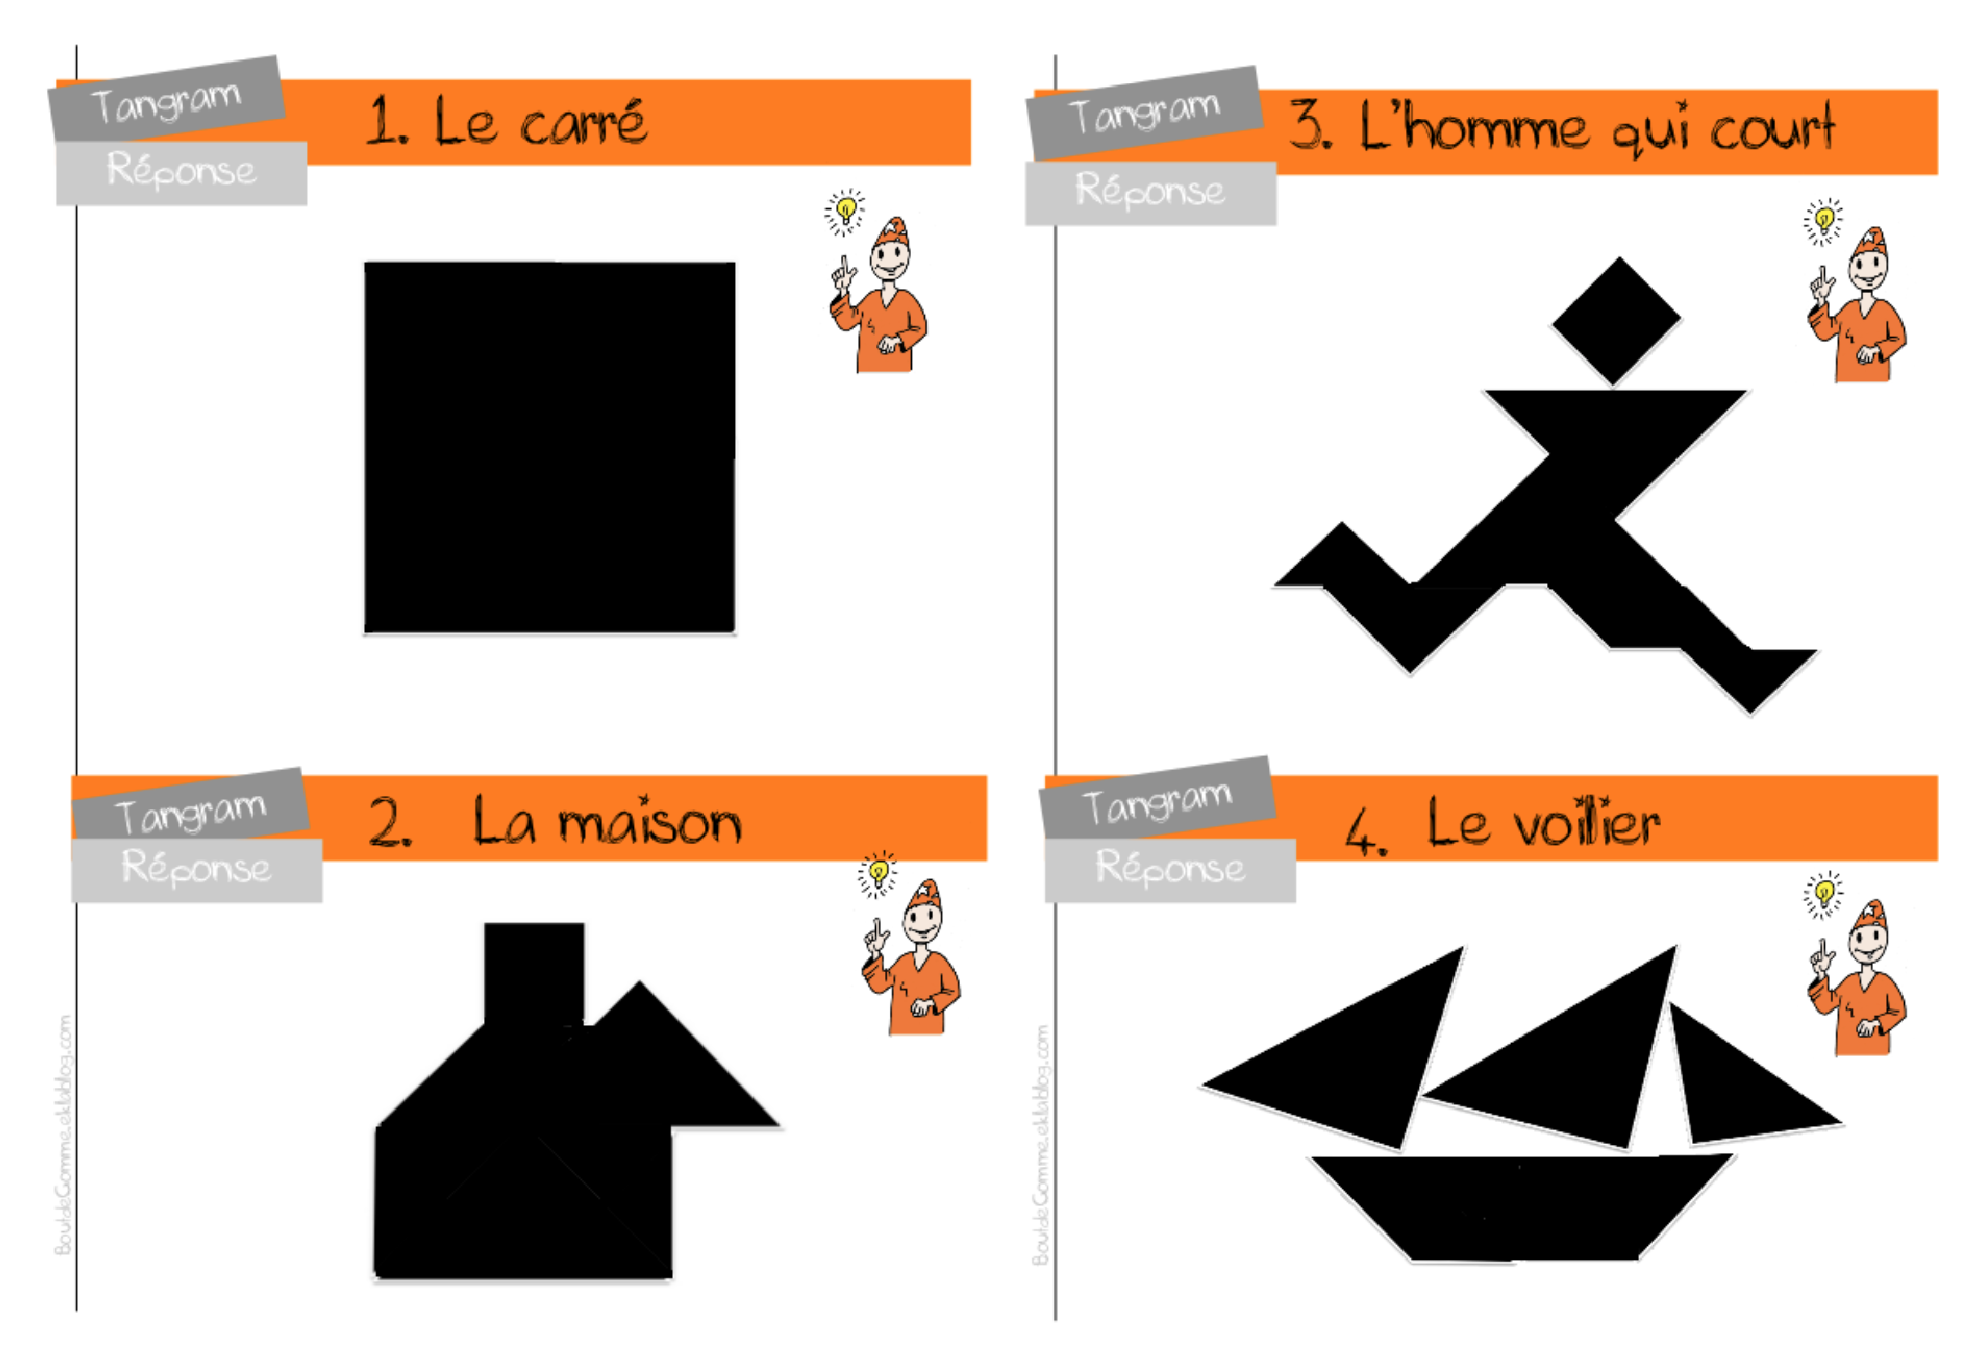
\includegraphics[width=16cm]{Geometrie_did/Images/Geo5_activite_rallye1} \\
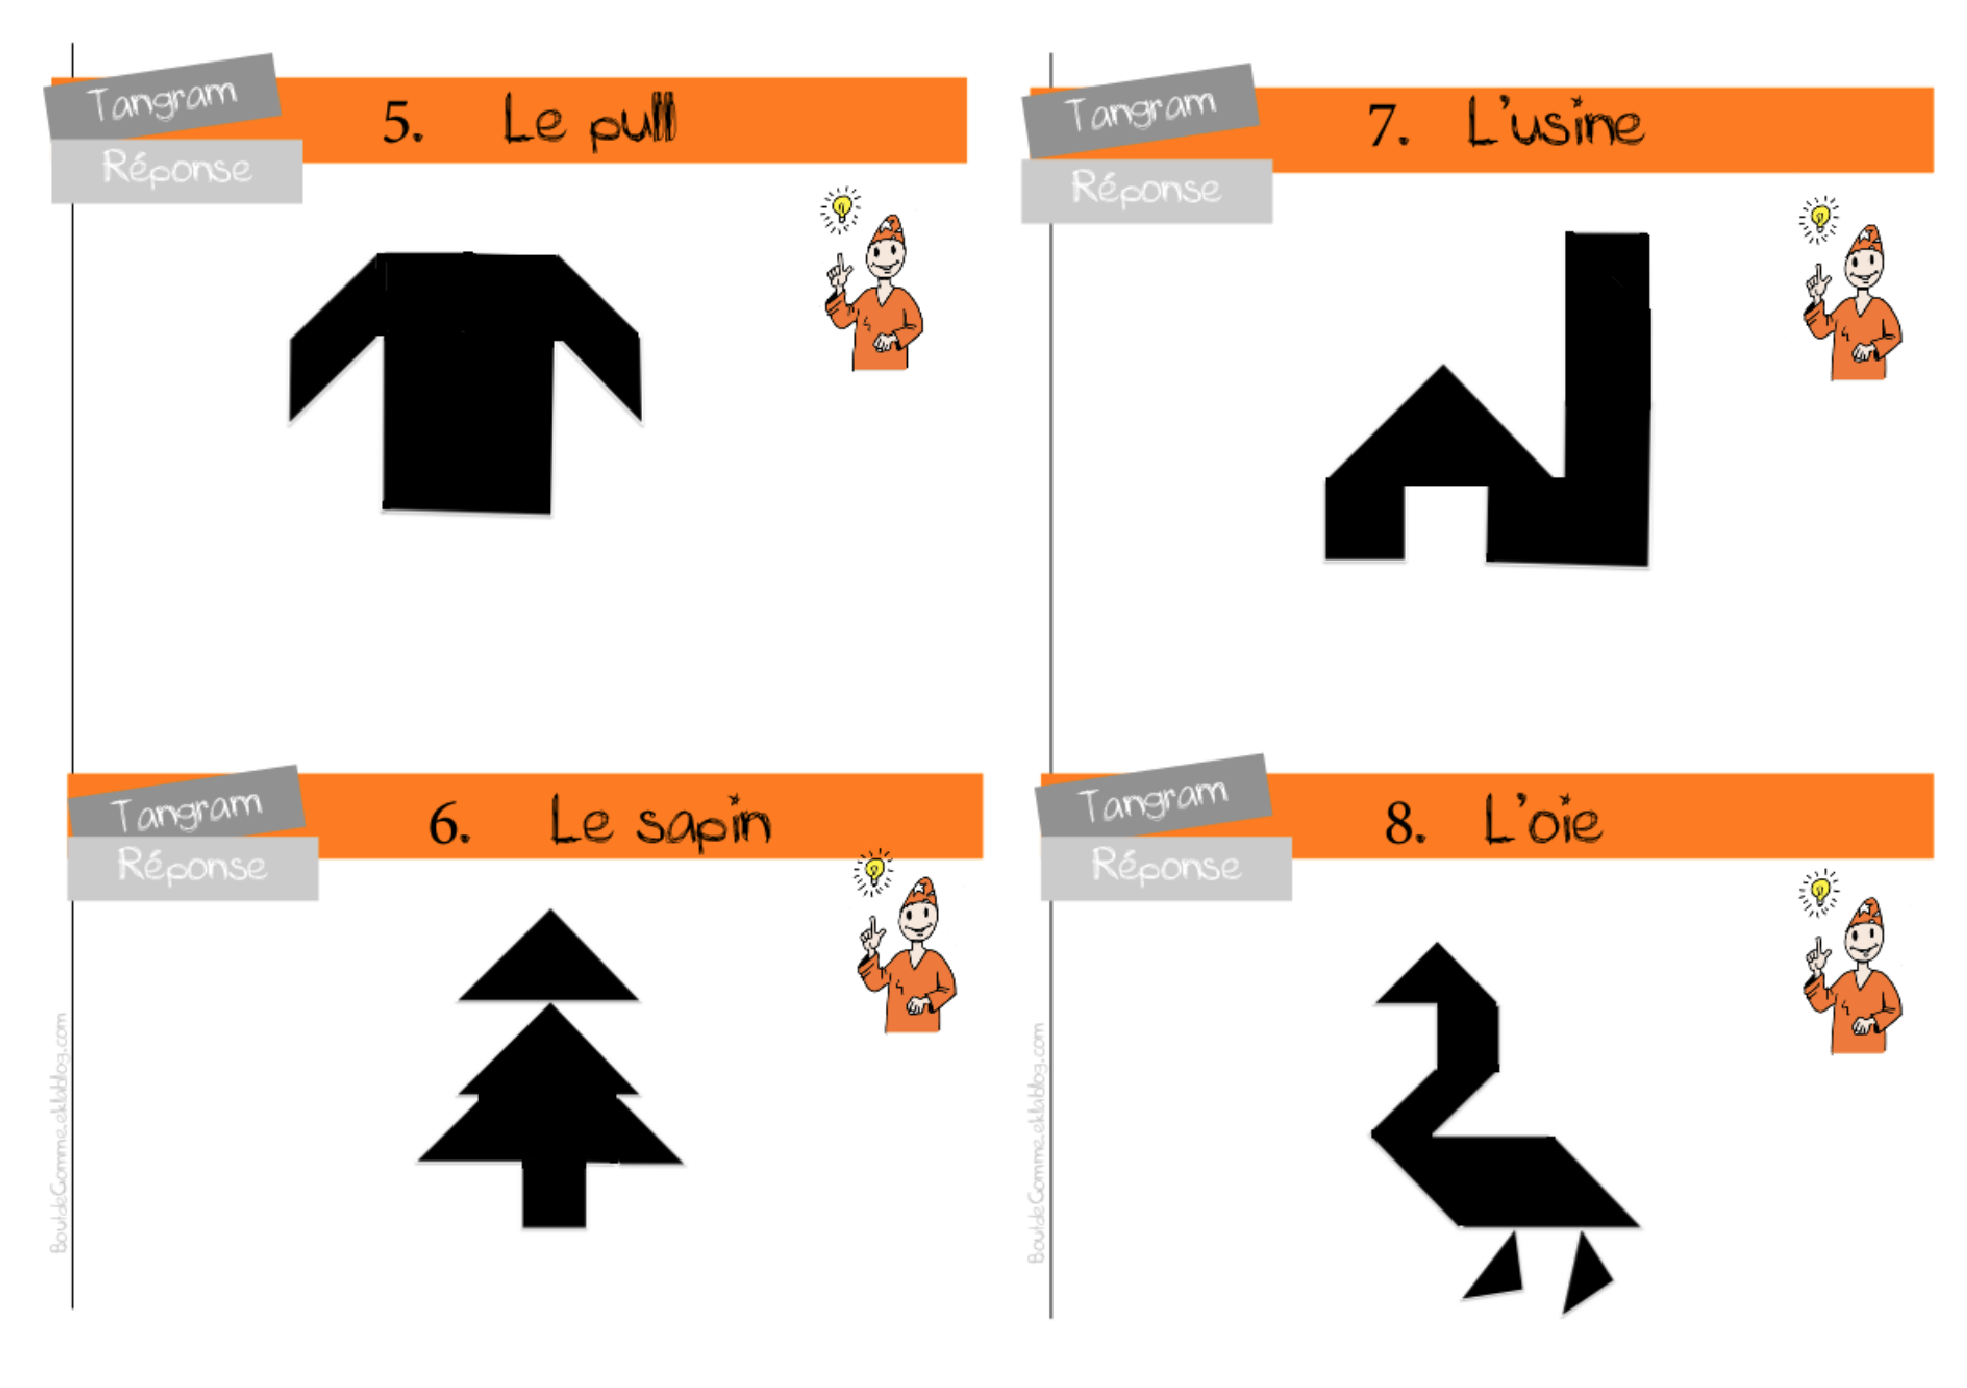
\includegraphics[width=16cm]{Geometrie_did/Images/Geo5_activite_rallye2}
\end{exercice*}



\begin{exercice*}[\fbox{C3} - Tangram, le retour !!!]
{\it La légende dit qu'un empereur chinois du 16\up{è} siècle du nom de « Tan », fit tomber un carreau de faïence qui se brisa en 7 morceaux. Il n'arriva jamais à rassembler les morceaux pour reconstituer le carreau mais l'homme s'aperçut qu'avec les 7 pièces il était possible de créer de formes multiples, d'où l'origine du jeu de tangram.} \\

Le tangram est un carré composé de 7 pièces :
\begin{itemize}
   \item 2 petits triangles rectangles isocèles ;
   \item 1 triangle rectangle isocèle de taille moyenne ;
   \item 2 grands triangles rectangles isocèles ;
   \item 1 carré ;
   \item 1 parallélogramme. \\
\end{itemize}

Les différentes exploitations pédagogiques du tangram (en géométrie, mais aussi en grandeurs et mesures) :
\begin{itemize}
   \item travail sur le vocabulaire des formes géométriques ;
   \item travail sur la description et la reproduction de figures sur feuilles quadrillées et unies ;
   \item travail sur la réalisation de programmes de construction ;
   \item travail sur les fractions ;
   \item travail sur la mesure et la comparaison de périmètres ;
   \item travail sur la mesure et la comparaison d’aires ;
   \item travail sur l’agrandissement/réduction\dots \\
\end{itemize}

\begin{center}
   {\textcolor{B1}{{\Large Un exemple de séquence en cycle 3}}}
\end{center}

{\bf Objectif de la séquence :} permettre aux élèves d’améliorer leur vision de l’espace (repérage, orientation), de se familiariser avec quelques figures planes et de passer progressivement d’une géométrie de la perception à une géométrie où les objets sont contrôlés par explication de propriétés et recours à des instruments. \\
On pourra faire les phases 1 à 3 dans une même séance et la phase 4 dans une deuxième séance. \\

{\bf Compétences visées :}
\begin{itemize}
   \item reconnaître de manière perceptive une figure plane, en donner le nom ;
   \item vérifier l'existence d'une figure simple en ayant recours aux propriétés et aux instruments ;
   \item décomposer une figure en figures plus simples ;
   \item tracer une figure (sur papier uni, quadrillé ou pointé), soit à partir d’un modèle, soit à partir d’une description, d’un programme de construction ;
   \item utiliser à bon escient le vocabulaire suivant : triangle, triangle rectangle, triangle isocèle, carré, parallélogramme. \\
\end{itemize}

{\bf Matériel :} la classe est organisée en ilots, chaque groupe disposant de quatre tangrams de couleurs différentes. \\

{\bf Phase 1 : découverte et manipulation du materiel.} \hfill {\it10 minutes} \\
La classe est organisée en groupes de quatre. On donne les quatre jeux de sept pièces de tangram de couleurs différentes à chaque élève et on les laisse manipuler et découvrir le matériel. \\
Dans un premier temps, pas de consigne précise si ce n’est d'essayer de ranger ces pièces en différentes catégories ou de construire des figures avec celles-ci. \\
Observer leurs actions : rangement par couleur, construction de figures ensemble, échanges de pièces\dots \\

{\bf Phase 2 : présentation et description du jeu.} \hfill {\it  15 minutes} \\
{\it Objectif de cette phase :} utilisation d’un vocabulaire mathématique précis, rappel des formes déjà connues à ce niveau (carré, triangle rectangle voir si possible triangle rectangle isocèle facile à repérer
par simple manipulation). \\
{\it Consigne :} le jeu que je vous ai distribué s’appelle le tangram. Il se constitue de sept pièces. Pouvez vous me les décrire ? Me donner leur nom ? \\
{\it Trace écrite :}
\begin{center}
\psframebox[framesep=2mm,fillcolor=yellow!20,
  fillstyle=solid,cornersize=absolute,linearc=.5\baselineskip]{\parbox{14.5cm}{
   \centering{\bf Le tangram comporte les sept pièces suivantes} \\
   \begin{pspicture}(-1,-0.5)(13.5,7.5)
      \psset{fillstyle=solid,fillcolor=white}
      \psframe(0,5)(2,7)
      \rput(1,6){\Large 1}
      \pspolygon(3,5)(5,5)(3,7)
      \rput(3.65,5.65){\Large 2}
      \pspolygon(6,5)(8,5)(6,7)
      \rput(6.65,5.65){\Large 3}
      \pspolygon(10,5)(12,5)(10,7)(8,7)
      \rput(10,6){\Large 4}
      \pspolygon(0,0)(4,0)(0,4)
      \rput(1.33,1.33){\Large 5}
      \pspolygon(5,0)(9,0)(5,4)
      \rput(6.33,1.33){\Large 6}
      \pspolygon(10,0)(12.83,0)(10,2.83)
      \rput(10.94,0.94){\Large 7}
   \end{pspicture}
   La figure 1 est un carré, \\
   les figures 2, 3, 5, 6 et 7 sont des triangles rectangles isocèles, \\
   la figure 4 est un parallélogramme.}}
\end{center}

\bigskip

{\bf Phase 3 : reproduction de figures.}  \hfill {\it 20 minutes} \\
{\it Objectif de cette phase :} reproduire une figure composée de figures simples. \\ [-3mm]

{\it Consigne 1 :} vous allez prendre les pièces 2 et 3 et vous allez reconstituer la figure 1 puis la figure 4. Enfin, avec ces deux mêmes pièces vous essaierez de faire un triangle plus grand, correspond-il au triangle 6 ou 7 ? \\
Faire reformuler la consigne en exigeant l’emploi du nom précis pour chaque figure. \\
Une fois que vous aurez reproduit ces trois figures, mettez les à coté et comparez les : que pouvez-vous en dire ? \\
{\it Configurations attendues :} \\
\begin{pspicture}(-2,4.5)(13,8)
   \psframe(0,5)(2,7)
   \psline(2,5)(0,7)
   \pspolygon(6,5)(8,5)(6,7)(4,7)
   \psline(6,5)(6,7)
   \pspolygon(10,5)(12.83,5)(10,7.83)
   \psline(10,5)(11.41,6.41)
\end{pspicture} \\
On peut faire remarquer que chacune des figures fait la même aire (la même surface) car elles sont toutes composées des
deux mêmes triangles\dots{} ce qui pourra faire l’objet d’une séance ultérieure sur ce thème. \\

{\it Consigne 2 :} vous allez reproduire la figure ci-dessous avec les figures 1,2,3,4 de trois manières différentes. \\
\begin{pspicture}(-6,0)(4,2.5)
   \pspolygon[fillstyle=solid, fillcolor=yellow!20](0,0)(4,0)(2,2)(0,2)
\end{pspicture} \\
{\it Configurations attendues :} \\
\begin{pspicture}(-1,-0.5)(4,2.5)
   \pspolygon(0,0)(4,0)(2,2)(0,2)
   \psline(2,0)(2,2)
\end{pspicture}
\begin{pspicture}(-1,-0.5)(4,2.5)
   \pspolygon(0,0)(4,0)(2,2)(0,2)
   \psline(2,0)(0,2)
\end{pspicture}
\begin{pspicture}(-1,-0.5)(4,2.5)
   \pspolygon(0,0)(4,0)(2,2)(0,2)
   \psline(0,0)(2,2)
\end{pspicture} \\
On Remarque que cette figure est égale à un carré et un petit triangle, un parallélogramme et un petit triangle, un moyen triangle et un petit triangle soit une aire correspondant à trois petits triangles. \\ [-3mm]

{\it Consigne 3 :} vous allez reproduire la figure 5 (ou 6) de trois manières différentes en vous servant des figures 1, 2, 3 et 4. Laisser le temps aux élèves de chercher puis conclure en les présentant au tableau. \\
{\it Configurations attendues :} \\
\begin{pspicture}(0,0)(6,3)
   {\psset{unit=1.414}
   \pspolygon(0,0)(4,0)(2,2)
   \psline(1,1)(2,0)(3,1)}
\end{pspicture}
\begin{pspicture}(0,0)(6,3)
   {\psset{unit=1.414}
   \pspolygon(0,0)(4,0)(2,2)
   \psline(1,1)(2,0)(2,2)}
\end{pspicture}
\begin{pspicture}(0,0)(6,3)
   {\psset{unit=1.414}
   \pspolygon(0,0)(4,0)(2,2)
   \psline(2,0)(1,1)(3,1)}
\end{pspicture} 

{\it Consigne 4 :} trouver un maximum de manières différentes pour faire la figure suivante avec les pièces 1, 2, 3, 4, 7. \\
\begin{pspicture}(-7,0)(4,2.5)
   \pspolygon[fillstyle=solid, fillcolor=yellow!20](-2,0)(4,0)(2,2)(0,2)
\end{pspicture} \\
Donner la silhouette de la figure et tracer les traits manquant selon la ou les solutions que vous avez trouvées. \\
{\it Configurations attendues :} \\
\begin{pspicture}(-3,-0.5)(6,2.5)
   \pspolygon(-2,0)(4,0)(2,2)(0,2)
   \psline(0,0)(0,2)
   \psline(2,0)(2,2)
\end{pspicture}
\begin{pspicture}(-2,-0.5)(5,2.5)
   \pspolygon(-2,0)(4,0)(2,2)(0,2)
   \psline(0,0)(2,2)
\end{pspicture}
 \\
 \begin{pspicture}(-3,0)(6,2)
   \pspolygon(-2,0)(4,0)(2,2)(0,2)
   \psline(0,2)(0,0)(2,2)
\end{pspicture}
\begin{pspicture}(-2,0)(5,2)
   \pspolygon(-2,0)(4,0)(2,2)(0,2)
   \psline(0,0)(2,2)(2,0)
\end{pspicture} 

{\bf Phase 4 : la construction du tangram.} \hfill {\it 45 minutes} \\
{\it Objectif de cette phase :} construire une figure complexe à partir de figures simples, élaborer un programme de construction. \\ [-3mm]

{\it Consigne 1:} essayer maintenant avec les pièces dont vous disposez de réaliser le tangram, c'est à dire le grand carré. \\
{\it Configuration attendue :} \\
{\psset{unit=1.414}
\begin{pspicture}(-3.5,-0.5)(4,4)
   \psframe(0,0)(4,4)
   \psline(0,0)(4,4)
   \psline(3,1)(0,4)
   \psline(2,0)(4,2)
   \psline(2,0)(1,1)
   \psline(3,1)(3,3)
   \rput(0.8,2){\large 5}
   \rput(2,3.2){\large 6}
   \rput(1,0.4){\large 2}
   \rput(2,1){\large 1}
   \rput(2.6,2){\large 3}
   \rput(3.5,2.5){\large 4}
   \rput(3.5,0.6){\large 7}
\end{pspicture}}

{\it Consigne 2 :} tracer le tangram sur une feuille quadrillée ou à petits carreaux. Le grand carré doit mesurer 8 cm de côté.
Variante plus difficile : construire le tangram sur une feuille unie. \\

{\it Consigne 3:} établir un programme de construction. \\
Variante plus facile : on pourra indiquer sur le tangram le nom des points à utiliser dans le programme. \\

\begin{minipage}{9.5cm}
{\psset{unit=2}
\begin{pspicture}(-0.25,-0.25)(4.25,4.25)
   \psgrid[subgriddiv=2,gridlabels=0,gridcolor=lightgray](0,0)(4,4)
   \psframe(0,0)(4,4)
   \psline(0,0)(4,4)
   \psline(3,1)(0,4)
   \psline(2,0)(4,2)
   \psline(2,0)(1,1)
   \psline(3,1)(3,3)
   \rput(-0.15,4.15){A}
   \rput(4.15,4.15){B}
   \rput(4.15,-0.15){C}
   \rput(-0.15,-0.15){D}
   \rput(4.15,2){E}
   \rput(2,-0.15){F}
   \rput(3.15,0.85){G}
   \rput(2,1.8){H}
   \rput(3,3.2){I}
   \rput(1,1.2){J}
\end{pspicture}}
\end{minipage}
\begin{minipage}{7.5cm}
{\it Exemple de programme :}
\begin{enumerate}
   \item tracer un carré ABCD de 8 cm de côté ;
   \item tracer la diagonale [BD] ;
   \item placer le point E, milieu du segment [BC] et le point F, milieu du segment [CD] ;
   \item tracer le segment [EF] ;
   \item placer le point G, milieu du segment [EF] ;
   \item tracer le segment [AG] ;
   \item placer H, le point d’intersection des segments [AG] et [BD] ;
   \item placer le point I, milieu du segment [HB] ;
   \item tracer le segment [GI] ;
   \item placer le point J, milieu du segment [DH] ;
   \item Tracer le segment [FJ].
\end{enumerate}
\end{minipage}
\end{exercice*}   

